\documentclass[12pt,a4paper]{report}
\usepackage[english]{babel}
\usepackage[T1]{fontenc}
\usepackage{times}
\usepackage{amsmath}
\usepackage{amsfonts}
\usepackage{amssymb}
\usepackage{textcomp}
\usepackage{gensymb}
\usepackage{hyperref}
\usepackage{graphicx}
\usepackage{tikz}
\usepackage{setspace}
\usepackage{mhchem}
\usepackage[left=2cm,right=2cm,top=2cm,bottom=2cm]{geometry}
\title{Interpolation of component characteristic maps for thermodynamic cycle assessment}
\author{Martin Heylen}
\newcommand{\citep}[1]{\cite{#1}}
\newcommand{\vect}[1]{\boldsymbol{#1}}

\begin{document}

\maketitle

\tableofcontents
\listoffigures
\listoftables
%%%%%%%%%%%%%%%%%%
%% Chapter 1:   %%
%% Introduction %%
%%%%%%%%%%%%%%%%%%
%\input{Chapter1_introduction}
\setstretch{1.5}
\chapter{Introduction}

\newpage
%%%%%%%%%%%%%%%%%%%%%%%%%%%%%%%%%
%% Chapter 2:                  %%
%% Notion of thermodynamics    %%
%%%%%%%%%%%%%%%%%%%%%%%%%%%%%%%%%
\chapter{Notions of thermodynamics}
\quad\; In the introduction, it has been introduced many times the concept and the used of the Brayton cycle. As explained, this concept has been applied for many usages, including electricity production and aircraft propulsion which are the most common and known applications.

It has been exposed that from the invention proposed by George Brayton in the end of the 19th century, the technology did really evolve.

Indeed, while the Brayton cycle engine first appears as a  piston engine where the compression, combustion and expansion occurs in the same enclosure, Nowadays 
the process is shared between at least three components (namely the compressor, the turbine and the combustion chamber).\\

However, what the previous did not cover were the keys notions to understand how theses components behave. Those notions, which will be used during this work, need to be defined and explained to allows to the common person to understand this writing without possessing those knowledge a priory. 

This problematic will be covered by this chapter, which will introduce step-by-step those notions.

\section{Fundamental notions}
\quad\; As mention in the lead-in of this chapter, the first sections of this report will entirely be devoted to the bringing in of the required knowledge for the understanding of the full report.

Starting from very fundamental notions, those will allow to explain more complex concept that will be applied in this work.

\subsection{Open/closed system}
The thermodynamic is a science that "studies the exchange of energy between a system and its environment or surrounding" \cite{thermoApp_1}.

The system is defined as being the area of the space selected for the study. Between the system and the environment lies the boundary. This boundary can either be real or fictitious and, can be static or mobile.\\

When the system is characterised, it has to be established if it is an open or a closed system.

The open systems are ones where a volume 

\newpage
%%%%%%%%%%%%%%%%%%%%%%%%%%%%%%%%%
%% Chapter 3:                  %%
%% Thermodynamics components   %%
%%%%%%%%%%%%%%%%%%%%%%%%%%%%%%%%%
\graphicspath{{Chapter_3_-_Thermodynamic_components/Images/}}
\chapter{Thermodynamic components}
\quad\, In the beginning of the previous chapter, it has been mention that the Brayton cycle composed of several components that are more or less complex. The behavior of these components, which is required to realized the study the global system, is based on the thermodynamic notions that have be introduce all along the past lines.

This chapter will be focused on the description of those components. For each of them, it will be provided the concepts or principles that will be used during this work. 
%% Turbomachines
\graphicspath{{Chapter_3_-_Thermodynamic_components/Images/}}
\section{Turbomachines}
\quad\, The first family of components to be studied is the turbomachines. The machines owning to this family are ones "that exchange energy between the
fluid traversing it and mechanical energy supplied to or extracted from the machine" \cite{Hillewaert2019}. Those machines are \textbf{rotating} machines and, based on the compressible nature of the fluid, two categories can be created.
This subsection will swept the two categories but will mainly focused on the machines exchanging energy with \textbf{compressible} flow.

\subsection{Incompressible flow}
\quad\, The first category of flow to be considered is the incompressible flow. This type of flow is characterized by a constant density over the distance. An example of incompressible fluid is the water.

Among the machine exchanging energy with such type of fluid, there are pumps which are designed to raise the height or total hydraulic energy $h$ of the fluid. The variation of the height of the fluid is similar to its enthalpy variation. Thus, the power output  $\dot{W}_p$ developed by the pump can be expressed as given in relation (\ref{eq:C3_Ppump})
\begin{equation}
\dot{W}_{p,a-b} = \dot{m}\cdot (h_a - h_b)=\dot{m}\cdot\Delta h_p \label{eq:C3_Ppump}
\end{equation}
considering that the transformation makes the system going from state \textbf{a} to state \textbf{b}.

If the consumed power of the pump is $\dot{W}_{e,a-b}$, its global efficiency $\eta_p$ is equal to the ratio
\begin{equation}
\eta_p = \frac{\dot{W}_{p,a-b}}{\dot{W}_{e,a-b}}\label{eq:C3_Etapump}
\end{equation}
\subsubsection{Characteristic maps}
\quad\, It has be shown that the power output and the global efficiency of the pump are functions of the height variation and the flow rate of the fluid. When operating a pump, it can be useful to know how this height variation will vary with respect to the flow rate and the rotational speed of the pump shaft. The knowledge of these two parameters allows to fully characterized the pump.

Considering the volumetric flow rate $Q_p$ (m$^3$/s) and the rotational speed $N$, the two following relations (\ref{eq:C3_DHp}) and (\ref{eq:C3_Pe}) can be derived.

\begin{subequations}
\setstretch{1}
\begin{equation}
\Delta h_p = \Delta h_p(Q_p, N)\label{eq:C3_DHp}\\
\end{equation}
\begin{equation}
\dot{W}_e = \dot{W}_ef(Q_p, N)\label{eq:C3_Pe}
\end{equation}
\end{subequations}
Those relations will be called characteristic or performance Map and are determined \textbf{experimentally}. An example of such map is given on Figure \ref{fig:C3_MapPump}.
\begin{figure}[h]
\centering
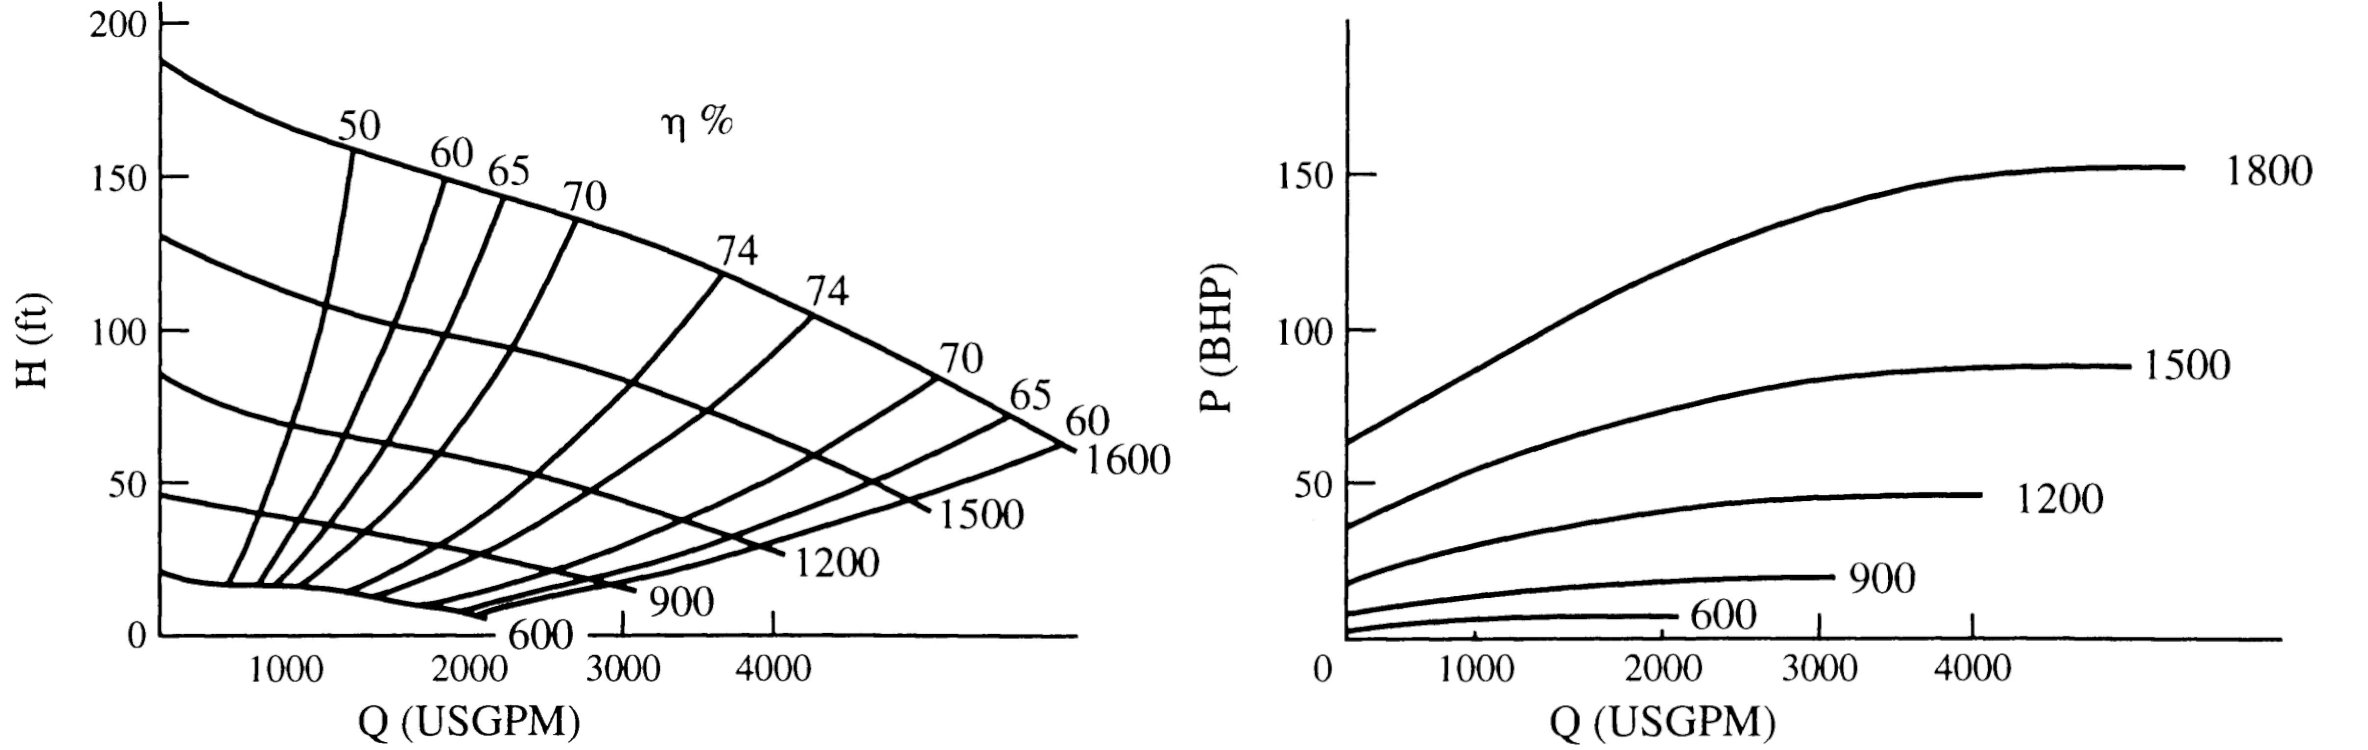
\includegraphics[width=0.8\textwidth]{char_map_pump.png}
\caption{Characteristic maps of a pump \citep{Hillewaert2019}}
\label{fig:C3_MapPump}
\end{figure}
\subsubsection{Similarity}
\quad\, When considering incompressible flow, it is possible to extrapolate from a known operating point a infinity of similar operating points. Indeed, There exist relationships which provides with enough accuracy the change of flow rate $Q$ and height variation $\Delta H$ when the rotational speed goes from $N_1$ to $N_2$. It can be demonstrate that the flow rate evolves linearly with the rotation speed, and that the height variation is a quadratic function of $N$.

\begin{subequations}
\setstretch{1}
\begin{equation}
Q_2 = Q_1\cdot\frac{N_2}{N_1} \label{eq:C3_Qsim}
\end{equation}
\begin{equation}
\Delta h_2 = \Delta h_1\cdot\left(\frac{N_2}{N_1}\right)^2 \label{eq:C3_DHsim}
\end{equation}\label{eq:C3_sim}
\end{subequations} 

These relations are really useful to extrapolate the performance maps of a pump. Similar relations can be deduced considering the variation of the radius of the pump.

One important property to notice is that all the dimensionless variables (e.g. the efficiency) are kept constant for all the different similar operational points. This is a valuable property which will be very useful for the future developments of the thesis.
\subsubsection{Types of pumps}
\quad\, Now that the exterior characteristics of the pumps have been defined, it is interesting to have at least a brief idea about how the pump is constructed. Without entering into detailed\footnote{see the section 4.3 and 4.4 of the course \citep{Hillewaert2019}}, there are two types of pumps.

The first type to be considered is the centrifugal pumps designed to provide a high heat for a low flow rate. Those pumps are characterized by an axial inflow and a radial outflow. The Figure \ref{fig:C3_centri_pump} shows a schematic of a centrifugal pumps.
\begin{figure}[h]
\centering
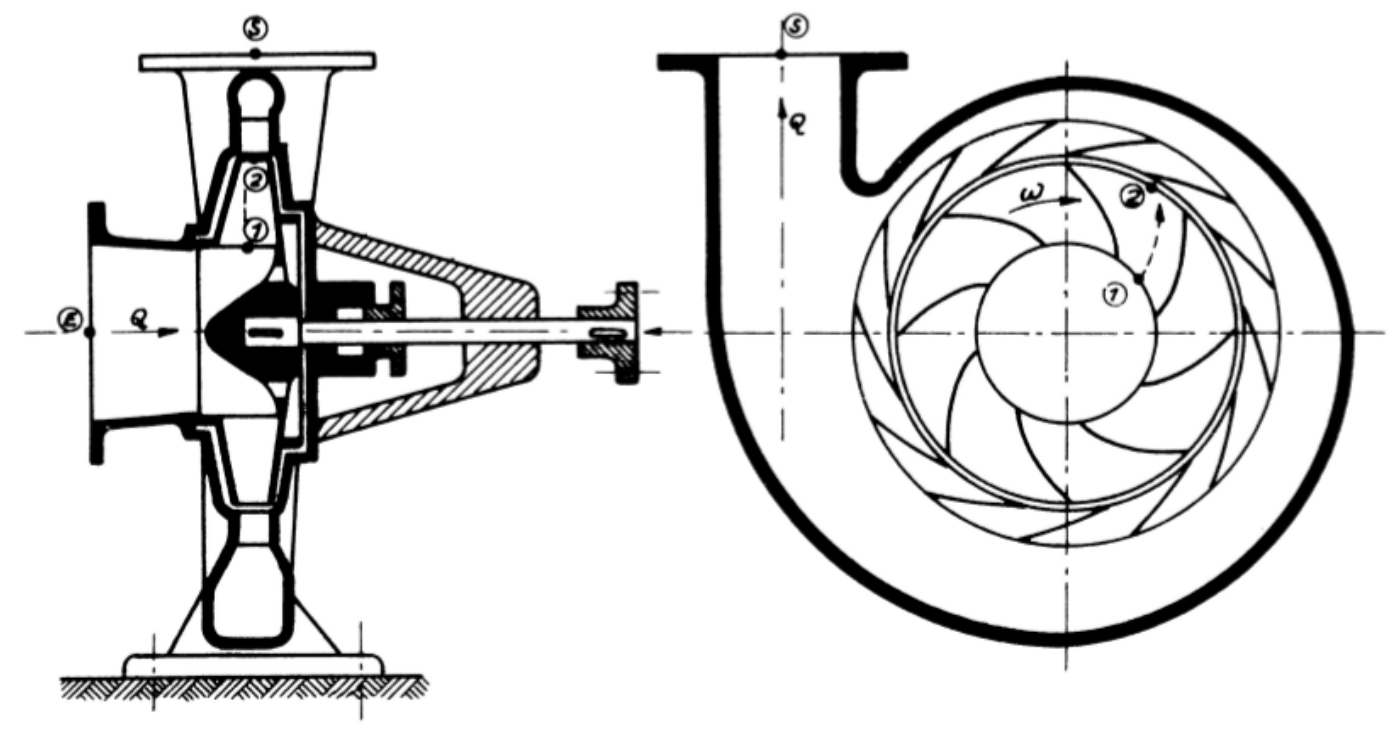
\includegraphics[width=0.4\textwidth]{centri_pump.png}
\caption{Centrifugal pump \citep{Hillewaert2019}}
\label{fig:C3_centri_pump}
\end{figure}

Basically, the centrifugal pump can be decomposed into two parts (for the most simple device). The first  part is the rotating impeller that will convert and transfer the mechanical energy to the fluid. Behind the impeller will be placed the volute (right picture of Figure \ref{fig:C3_centri_pump}) that collects the flow to bring it to the outlet of the pump.\newpage

The second type of pump are the axial pumps which are, in opposition with the centrifugal pumps, designed to deliver low head for high flow rates. Such pumps is illustrated on Figure \ref{fig:C3_axial_pump}. 
\begin{figure}[h!]
\centering
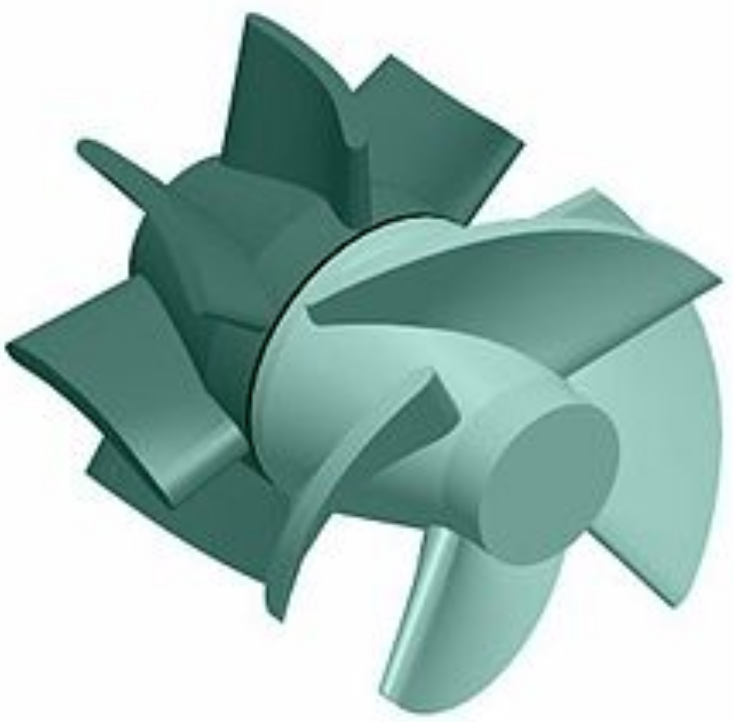
\includegraphics[width=0.25\textwidth]{axial_pump.png}
\caption{Axial pump \citep{Hillewaert2019}}
\label{fig:C3_axial_pump}
\end{figure}

The main two parts of an axial pumps are the rotor (the rotating part) that will increase the height of the fluid followed by a diffusor which "recuperates the kinetic energy at the exit of the rotor"\citep{Hillewaert2019}.

\subsection{Compressible flow}
\quad\, The previous subsection introduced the pump which is a turbomachine design to increase the energy of the incompressible fluid passing through it. However, this type of machine cannot deals with compressible flow for which the density can vary over the distance. For instance, the air is a compressible fluid. 

The behavior of the compressible flow is more complex to describe compared to incompressible flow. Indeed, "compressible flow is characterized by the propagation of acoustic waves"\citep{Hillewaert2019}.   This part of the section about turbomachines will only focused on the very main principles required for the good understanding of this work.

\subsubsection{Static and total quantities}
\quad\, As it has be partly reveal in the previous lines, the flow characteristics are dependent on its velocity. The study of compressible flow did lead to the distinction between the static and total quantities. 

The static quantities are state variables (e.g. temperature, pressure,...) that are independent of the flow velocity. As for the total quantities, these are dependent of the flow velocity $V$. For instance, the total enthalpy is given by
\begin{equation}
h^0 = h + \frac{1}{2}\cdot v^2\label{eq:C3_h0}
\end{equation}
where the total quantity is identified by the superscript "0".

The total enthalpy can be defined as "the static enthalpy obtained when the gas is brought adiabatically to a halt"\citep{Hillewaert2019}.


\subsubsection{Conservation of the total enthalpy and rothalpy}
\quad\, For an adiabatic transformation without viscous work, the total enthalpy is conserved between the initial state and the final state.
\begin{equation}
\dot{m}\cdot h_1^0 = \dot{m} h_2^0 \label{eq:C3_hcons}
\end{equation}
which can be reduced to $h_1^0 = h_2^0$ if we supposed that the transformation is performed without any leakages. The states $1$ and $2$ are associated to the orthogonal boundaries to the flow of the selected control volume delimiting the studied system. 

Now, considering a rotating system (e.g. a rotor), the variation of the total enthalpy can be obtained by considering the modified Euler equation of turbomachinery
\begin{align}
\setstretch{1}
h_2^0 - h_1^0 = \frac{1}{2}\cdot &\left(v_2^2 - v_1^2\right) - \frac{1}{2}\cdot \left(wr_2^2 - wr_1^2\right) + \frac{1}{2}\cdot \left(ur_2^2 - ur_1^2\right)\label{eq:C3_Euler}\\
\text{with }& v = \left|\vect{v}\right|\quad\text{;}\quad  wr = \left|\vect{wr}\right|\quad\text{;}\quad ur= \left|\vect{ur}\right|\nonumber
\end{align}
where $\vect{ur}$, $\vect{v}$ and $\vect{wr}$ are respectively the local velocity of the rotor, and the absolute and relative velocity (with respect to the rotor) of the flow. Defining the total rothalpy as being 
\begin{equation}
i^0 = h + \frac{1}{2}\cdot wr^2 - \frac{1}{2}\cdot ur^2 \label{eq:C3_i0}
\end{equation}
It is obtained from the Euler equation (\ref{eq:C3_Euler}) that the total rothalpy is conserved through the transformation.
\begin{equation}
i_1^0 = i_2^0 \label{eq:C3_icons}
\end{equation}
\subsubsection{Velocity triangle}
\quad\, With the relation (\ref{eq:C3_Euler}), the notion of absolute and relative velocity of the flow has been introduced. A graphic representation of these three vector can be done using the \textbf{velocity triangle}. This triangle is drawn on Figure \ref{fig:C3_vtriang}.
\begin{figure}[h]
\centering
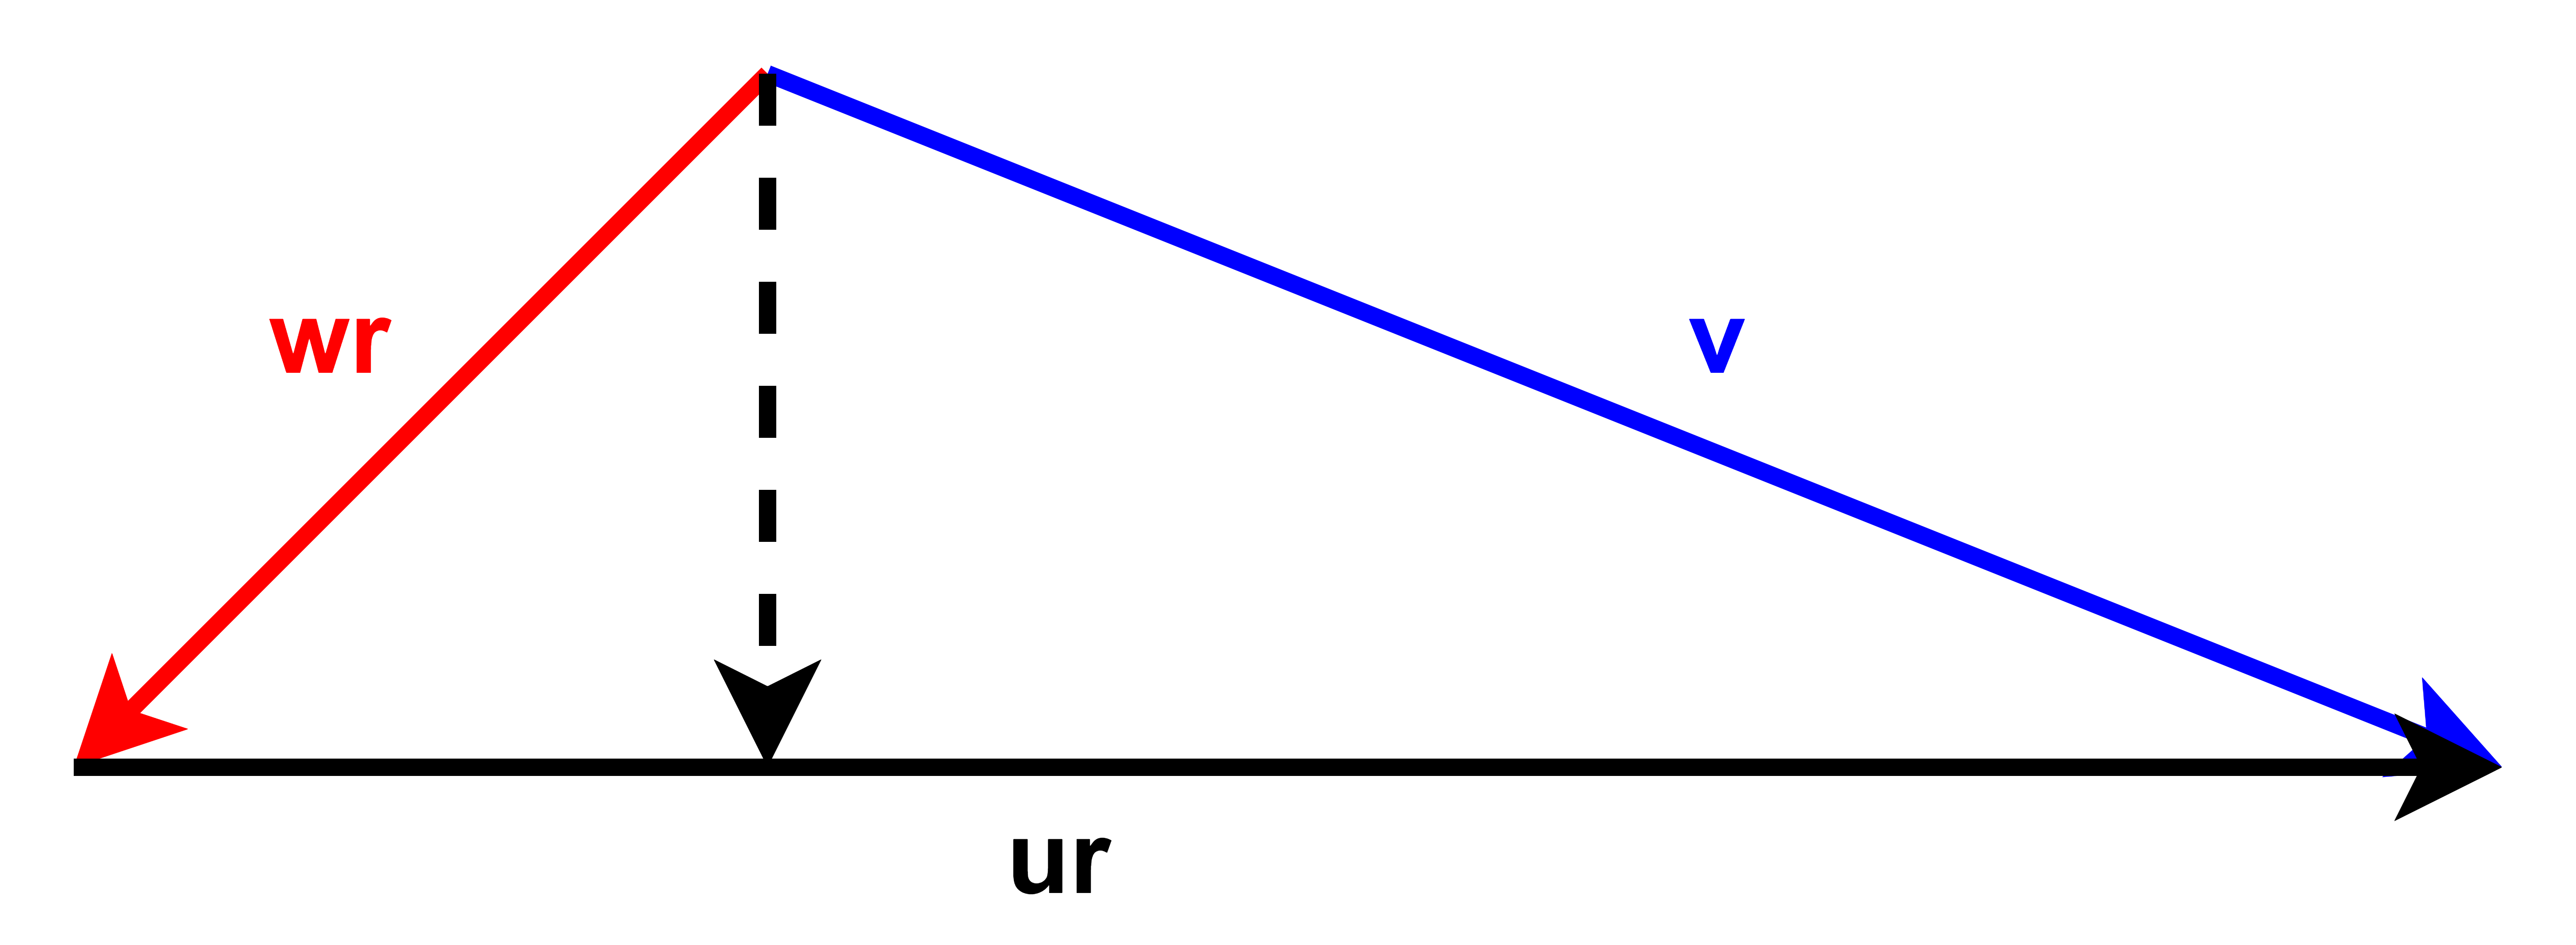
\includegraphics[width=0.6\textwidth]{Vtriangle.png}
\caption{Velocity triangle}
\label{fig:C3_vtriang}
\end{figure}

\subsubsection{Mach number}
The Mach number $M$ is defined as being the ratio between the velocity $v$ and the sound speed $a$.
\begin{equation}
M = \frac{v}{a} \label{eq:C3_Mach}
\end{equation}
The Mach number $M$ is a dimensionless variable that gives an image of the compressible effects of the flow. Thus, one criteria for the determination of similar operational points is to keep constant the Mach number.

Using the Mach number allows to obtain formulas to compute the total quantities base the static ones. By considering first the total temperature, it can be found
\begin{equation}
T^0 = T + \frac{v^2}{2\cdot c_p} = T\cdot\left(1 + \frac{v^2}{2\cdot c_p\cdot T}\right)\label{eq:C3_TT0_1}
\end{equation}
For an isentropic process, it can be demonstrate that the speed of sound $a=k\cdot r\cdot T$. Thus, the equation (\ref{eq:C3_TT0_1}) becomes
\begin{equation}
T^0 = T\cdot\left(1 + \frac{k-1}{2}\cdot M^2\right) = T\cdot f(M) \label{eq:C3_TT0}
\end{equation}
Using the equations (\ref{eq:C2_isrelPT}), (\ref{eq:C2_isrelrhoT}) and the definition of the function $f(M)$, the relations linking the static to the total pressure, density and speed of sound can be obtained as well.

\begin{subequations}
\setstretch{1}
\begin{equation}
p^0 = p\cdot f(M)^\frac{k}{k-1}\label{eq:C3_PP0}
\end{equation}
\begin{equation}
\rho^0 = \rho\cdot f(M)^\frac{1}{k-1}\label{eq:C3_rhorho0}
\end{equation}
\begin{equation}
a^0 = a\sqrt{f(M)} \label{eq:C3_aa0}
\end{equation}
\end{subequations}

\subsubsection{Characteristic maps}
\quad\, As for the turbomachines exchanging energy with incompressible flow, those dealing with compressible flow can also be fully characterized knowing a pair of independent operating parameters. The most usual parameters are

\begin{itemize}
\setstretch{1}
\item $\dot{m}_c$ (kg/s or lbs/min): It is the corrected mass flow rate.

\item $N$ (rpm): It is the rotational speed of the turbomachine shaft. 

\item $\Pi$ (-): It is the pressure ratio between the inlet and the outlet of the turbomachines. If the turbomachines is compressing the flow, the ratio is reverse to keep it greater than one.

\item $\eta$ (-): It is the isentropic efficiency of the machine.
\end{itemize} 

The corrected mass flow rate is defined as follows

\begin{equation}
\dot{m}_c = \dot{m}\cdot \sqrt{\frac{T}{T_{ref}}}\cdot\left(\frac{p_{ref}}{p}\right)\label{eq:C3_mc}
\end{equation}

with $T_{ref}$ and $p_{ref}$ being the reference temperature and pressure (all quantities being static).

Let's supposed now that the rotational speed and the corrected mass flow are known. Then, the two other quantities ($\Pi$ and $\eta$) can be calculated by evaluating the relationships (\ref{eq:C3_Pimap}) and (\ref{eq:C3_etamap}).

\begin{subequations}
\setstretch{1}
\begin{equation}
\Pi = \Pi(N, \dot{m}_c)\label{eq:C3_Pimap}
\end{equation}
\begin{equation}
\eta = \eta(N, \dot{m}_c)\label{eq:C3_etamap}
\end{equation}
\end{subequations}  
These relations can be established by the means of experimental measurements.
\subsection{Gas compressor}
\quad\, The previous lines shows some properties of compressible flows that add complexity to the analysis. Now, it is interesting to describe two types of turbomachines inducing a modification of the state of the flow. 

The first machines to be describe are the compressor. As for the pumps, the compressor can be axial or centrifugal.  The axial compressor are mainly composed of a rotating part (the rotor), followed by a non moving part (the stator) converting the the kinetic energy at exit of the rotor into pressure. A schematic of an axial compressor stage is given on Figure \ref{fig:C3_compstage}.

\begin{figure}[h]
\centering
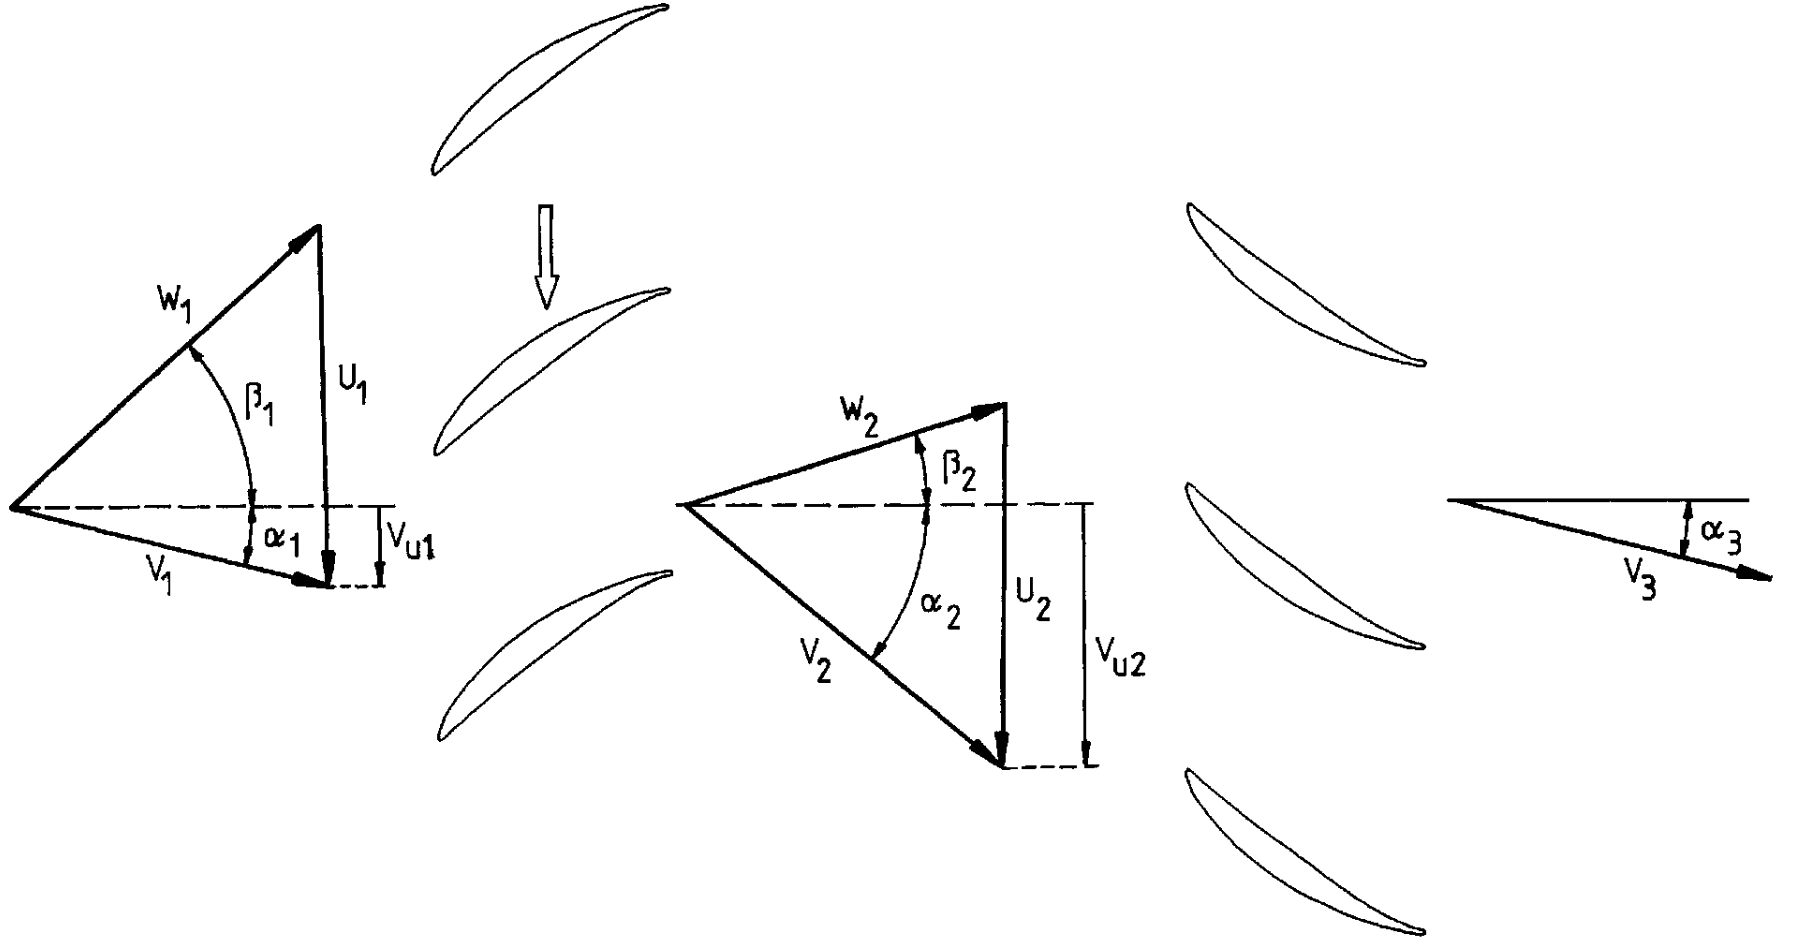
\includegraphics[width=0.5\textwidth]{Comp_stage.png}
\caption{Axial compressor stage \citep{Hillewaert2019}}
\label{fig:C3_compstage}
\end{figure}

The half-moon entities on the graph represent the blades of the rotor and stator (respectively the left and the right ones). It can be observed that the rotor blades increase the value of the flow velocity $v$. As explained earlier this augmentation of kinetic energy is then recovered by the stator blades. 

\subsubsection{Mollier diagram}
\quad\, The transformation induced by the compressor can be represented into a hs diagram also named \textbf{Mollier diagram}. The Mollier diagram for one compressor stage has been drawn on Figure \ref{fig:C3_Molliercomp}.

\begin{figure}[h]
\centering
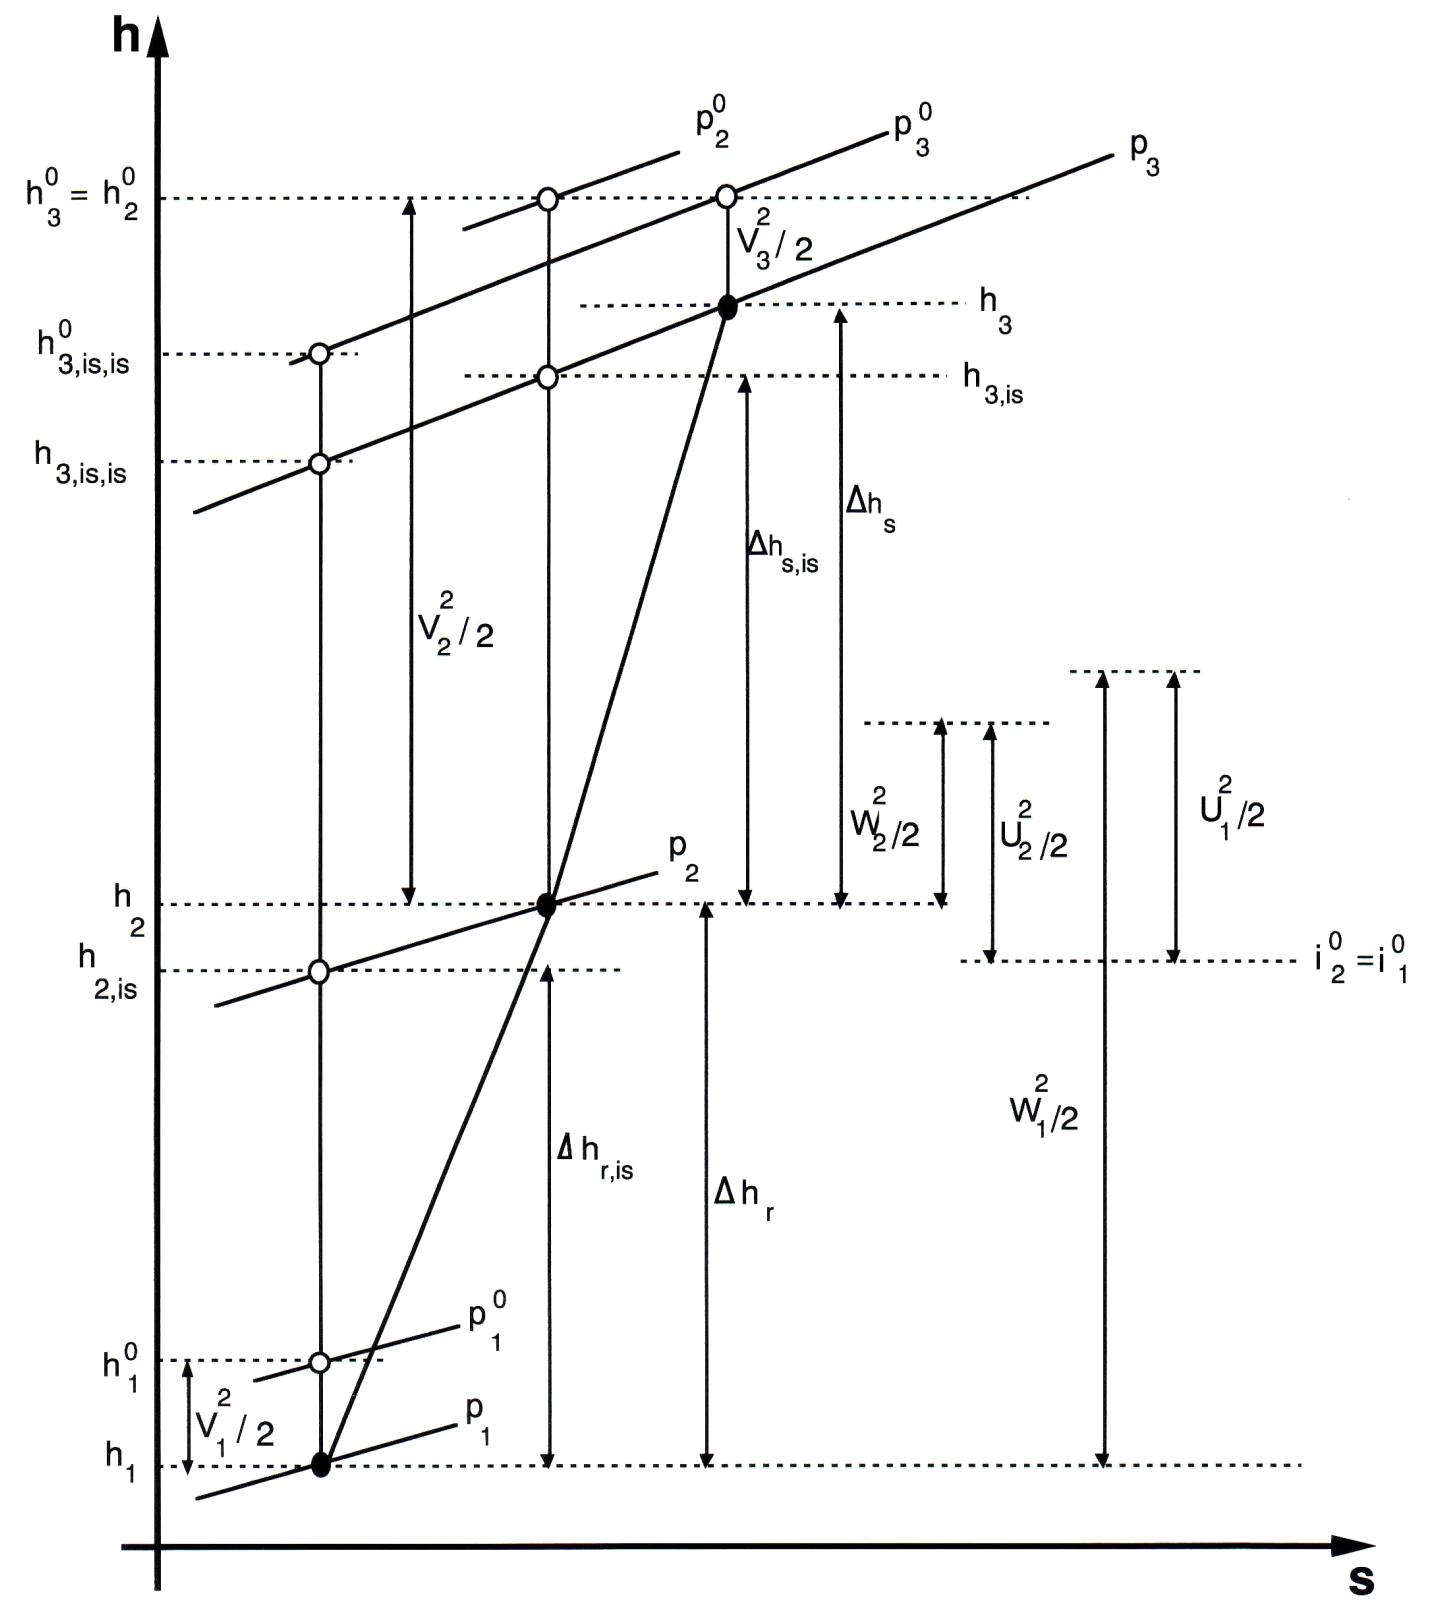
\includegraphics[width=0.5\textwidth]{Comp_mollier.png}
\caption{Mollier diagram of a compressor stage \citep{Hillewaert2019}}
\label{fig:C3_Molliercomp}
\end{figure}

The diagram, for which the velocity triangles are given on Figure \ref{fig:C3_compstage}, has to be read as follows.
\begin{itemize}
\setstretch{1}
\item State \textbf{1}: Starting from the static enthalpy and pressure $h_1$ and $p_1$, the relations (\ref{eq:C3_i0}), (\ref{eq:C3_h0}) and (\ref{eq:C3_PP0}) are used to calculate the total enthalpy, rothalpy and pressure.  
\item State \textbf{2}: The transformation \textbf{1}-\textbf{2} takes place within the rotor of the compressor stage. Thus, the total rothalpy is conserved over the transformation ($i_2^0=i_1^0$). 

The knowledge of the total rothalpy allows to determine the other quantities. The static enthalpy (and by extension the total enthalpy) can be deduced using the relation (\ref{eq:C3_i0}). Concerning the pressure, there is an increase of the static and total pressure of the fluid "due to the diffusion in the rotor passage"\citep{Hillewaert2019} ($p_2^{(0)} > p_1^{(0)}$).
 
\item State \textbf{3}: The transformation \textbf{2}-\textbf{3} takes place within the stator of the compressor stage. Thus, the total enthalpy is conserved over the transformation ($h_3^0 = h_2^0$).

Then, the static enthalpy can be computed using the relation (\ref{eq:C3_h0}). The conversion of the kinetic energy into pressure leads to an increase of the static and total pressure ($p_3^{(0)} > p_2^{(0)}$).
\end{itemize}
As it was mentioned in the subsection \ref{C2:Isen_eff}, the enthalpy at the end of the process is higher than the one considering an isentropic transformation.
\subsubsection{Performance maps}
\quad\, As for any turbomachines, the compressor can be characterized by its performance map. The map is composed of the performance plot often completed with the efficiency hill. The performance plot provides the total to total (TT) pressure ratio $\Pi_c$ as a function of the rotational speed $N$ and the corrected flow rate $\dot{m}_c$.

A illustration of a compressor performance map is given on Figure \ref{fig:C3_compmap}.
\begin{figure}[h]
\centering
\includegraphics[width=0.6\textwidth]{Comp_Map.png}
\caption{Illustration of a compressor performance map \citep{Ghorbanian2009}}
\label{fig:C3_compmap}
\end{figure}  

On the map, the solid and the dash curves represent respectively the iso-rotational speed and the iso-efficiency.

To remarkable lines are emphasized on the plot. For each rotational speed $N_c$, these lines provides minimal and maximal bound for the compressor pressure ratio $\Pi_c$. 

The lower limit is given by the choke line. "When the flow reaches the velocity at some cross-section"\citep{Ghorbanian2009}, an increase of the gas mass flow rate is not possible. Thus, the slope of the associated iso-rotational speed becomes equal to the infinity at this point. 

The upper bound is given by the "aerodynamic stability limit line" or surge line. At this minimal flow rate, the flow start to stall in the machine. Going beyond this limit would lead to a backward flow in the compressor, causing irreversible damages to the compressor. Thus when operating the machine, a certain margin is taken with respect to the surge line\footnote{For more information about the stall and surge events, sees section 9.5 of the course "Turbomachines" \citep{Hillewaert2019}}.

The compressor map, for the low rotational speeds, can be extrapolated by considering similar operational points. Indeed, for these low speed the approximation of considering an incompressible flow instead of a compressible is accurate enough. Though, the compressor can be assimilated to a pump and, using the relations of similarity \ref{eq:C3_sim}, the extrapolation is possible. 

\subsection{Gas turbine}
\quad\, From now, only compressors have been introduced. However, in a gas cycle, the compressor are combined with a turbine that will expand the gas. Only for some exception, the turbine is always placed after the combustion chamber. This choice allows to provide to the turbine a flow with very high enthalpy.

Typically, an axial gas turbine is composed of a stator followed by a rotor. The stator is design to create a deflection of the flow in the sens of rotation of the rotor. This will accelerate the flow before entering the rotor.

The schematic of an axial turbine stage is drawn on Figure \ref{fig:C3_turbstage}.
\begin{figure}[h]
\centering
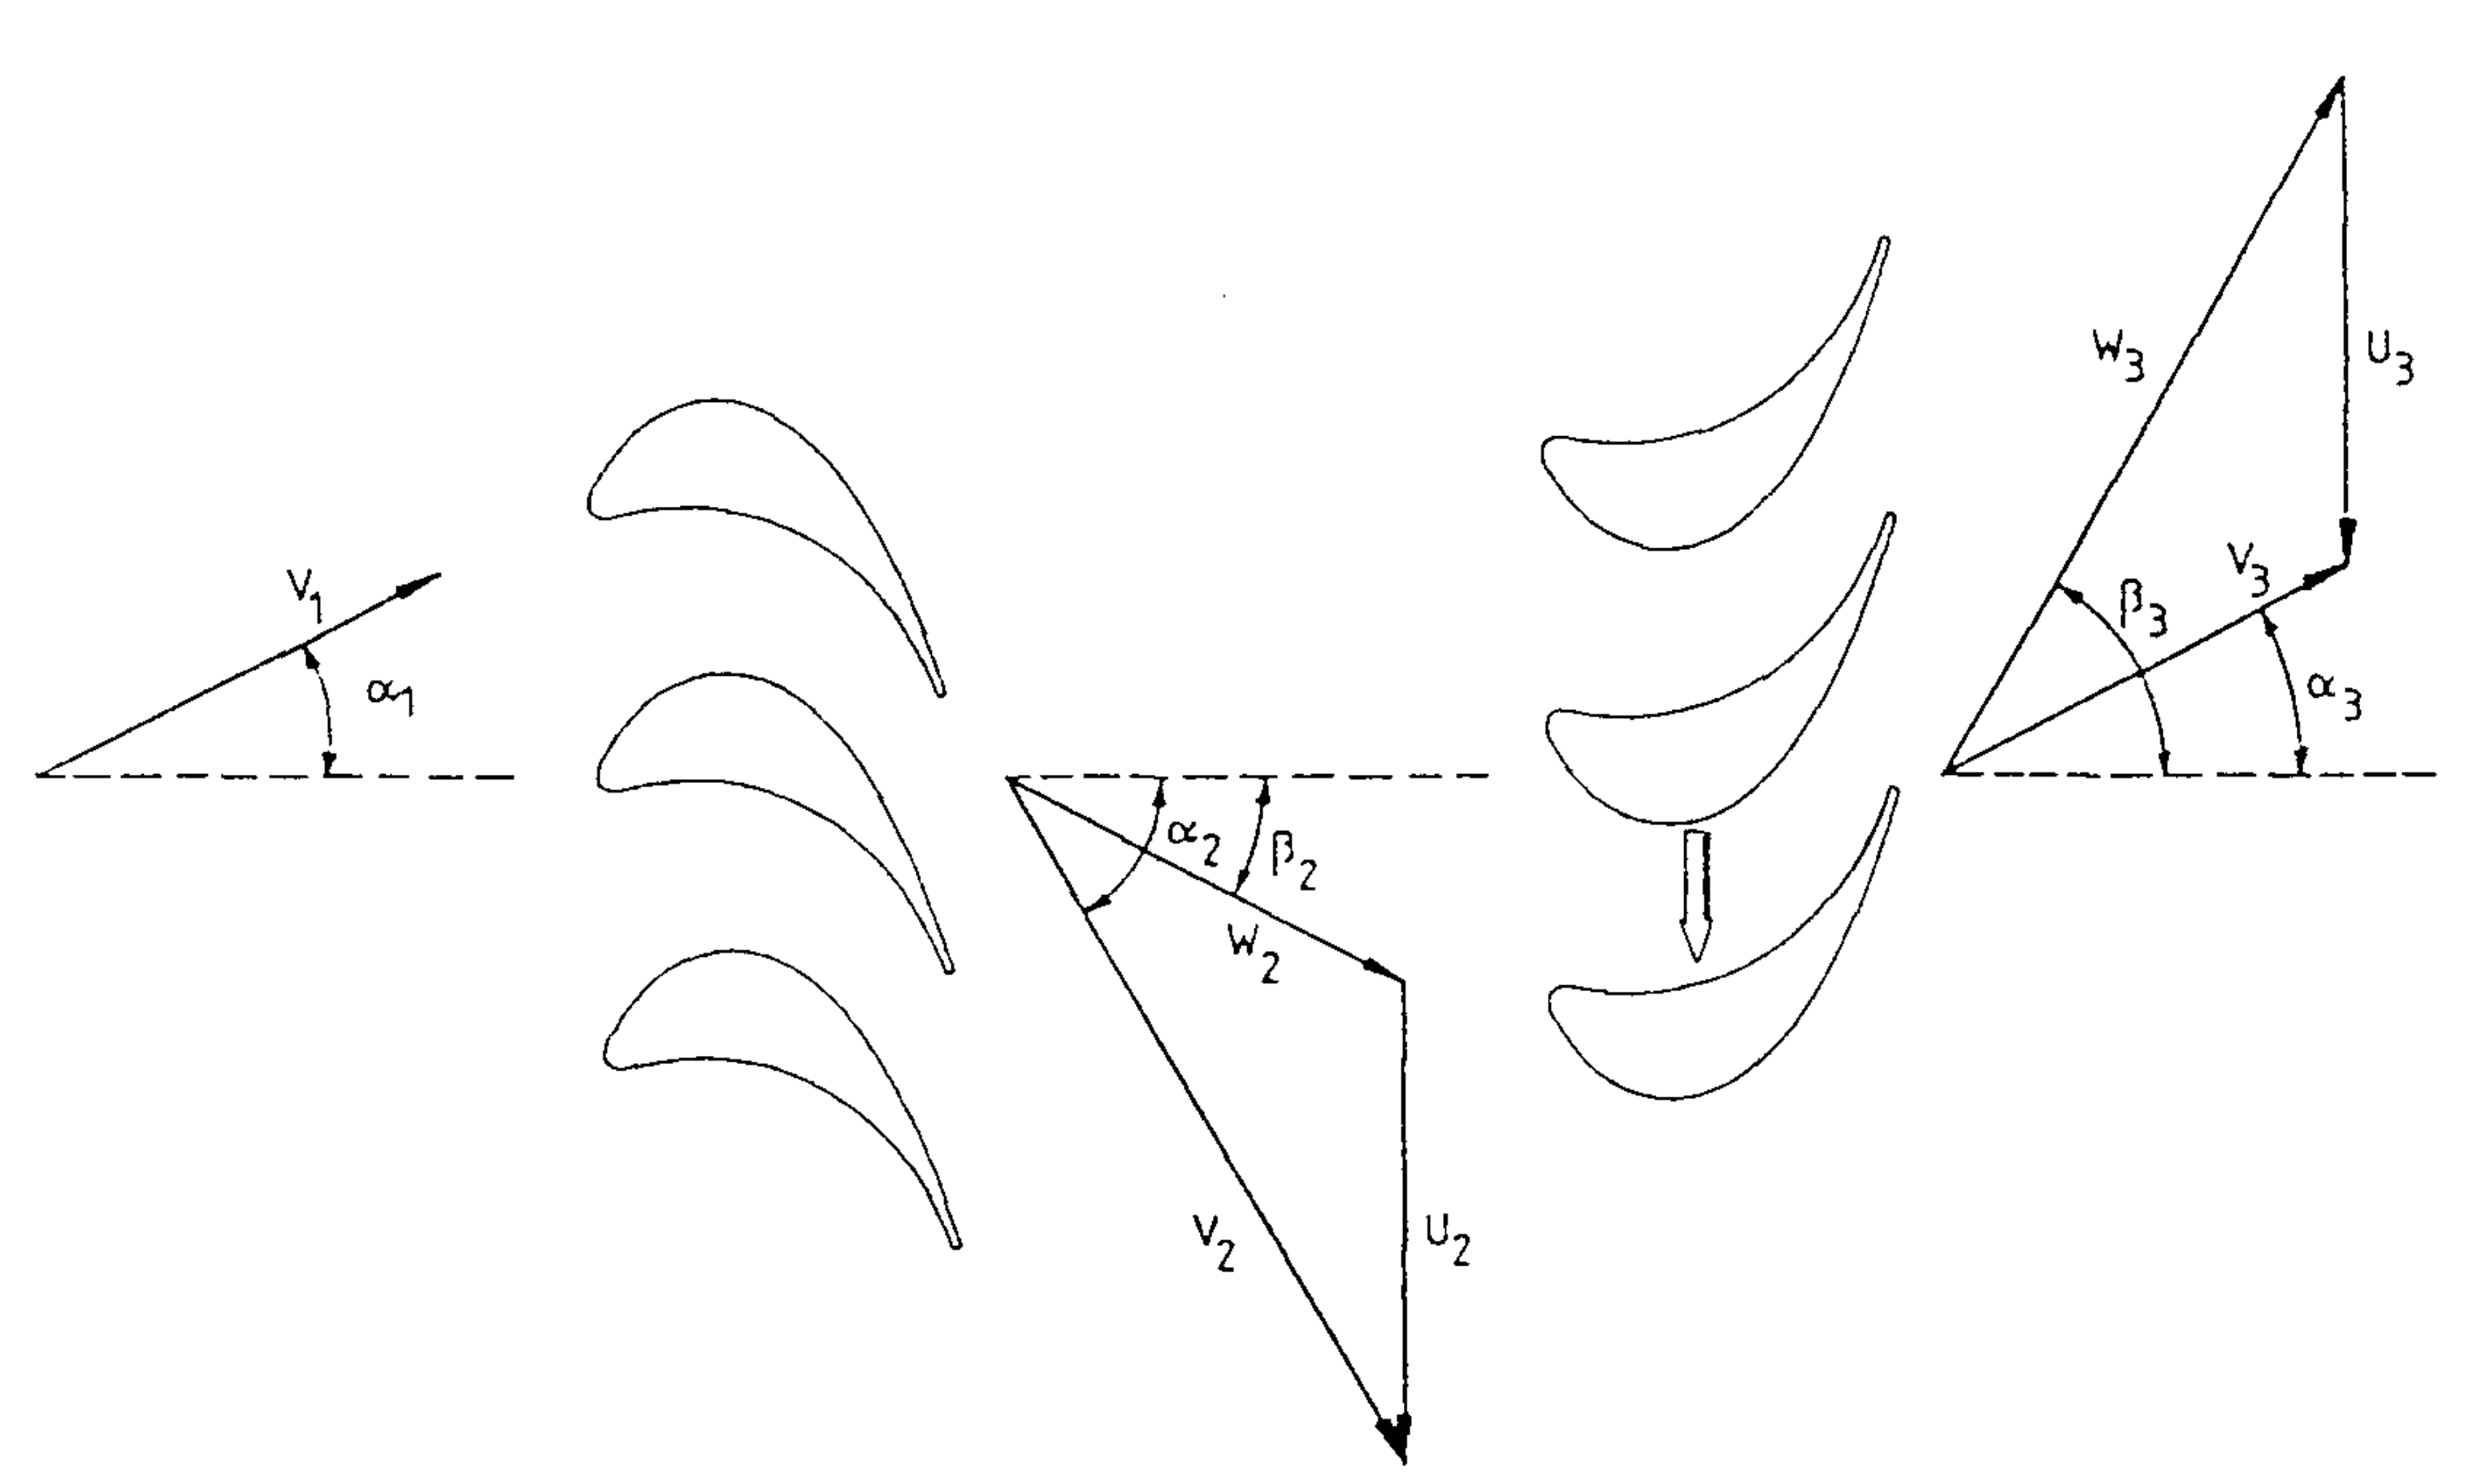
\includegraphics[width=0.5\textwidth]{Turb_stage.png}
\caption{Axial turbine stage \citep{Hillewaert2019}}
\label{fig:C3_turbstage}
\end{figure}

\subsubsection{Mollier diagram}
As for the compressor, the real expansion induced by the turbine can be represented into a Mollier diagram. The diagram is depicted on Figure \ref{fig:C3_Mollierturb}. The methodology to read the diagram is the same as before.


\begin{itemize}
\setstretch{1}
\item State \textbf{1}: Starting from the static enthalpy and pressure, the total quantities can be deduced.
\item State \textbf{2}: The transformation \textbf{1}-\textbf{2} takes place within the stator of the turbine stage. Therefore, the total enthalpy is conserved over the transformation ($h_2^0=h_1^0$). 

Knowing the total enthalpy of the state \textbf{2} allows to compute the static enthalpy and by extension the total rothalpy. Plus, since the flow is accelerated by the stator blades, the static and total pressure falls from state \textbf{1} to state \textbf{2} ($p_2^{(0)}<p_1^{(0)}$).
\item State \textbf{3}: The transformation \textbf{2}-\textbf{3} takes place within the rotor of the turbine stage. Therefore, the total rothalpy is conserved over the transformation ($i_3^0=i_2^0$).

Then, the relation (\ref{eq:C3_i0}) allows to retrieve the static enthalpy of state \textbf{3}. As shown on the schematic \ref{fig:C3_turbstage} of the turbine stage, the relative speed of the flow is augmented when going through the rotor passage. This generates a second drop of the static and total enthalpy and pressure ($p_3^{(0)}<p_2^{(0)}$). 

However, there exists special stage for which "the relative velocity of the flow to the blade row" of the rotor\citep{Hillewaert2019} remains unchanged, but the flow is inverted. Neglecting the very small variation of the rotor velocity, the static enthalpy and pressure remains unchanged when passing through the rotor.
\end{itemize} 

\begin{figure}[h]
\centering
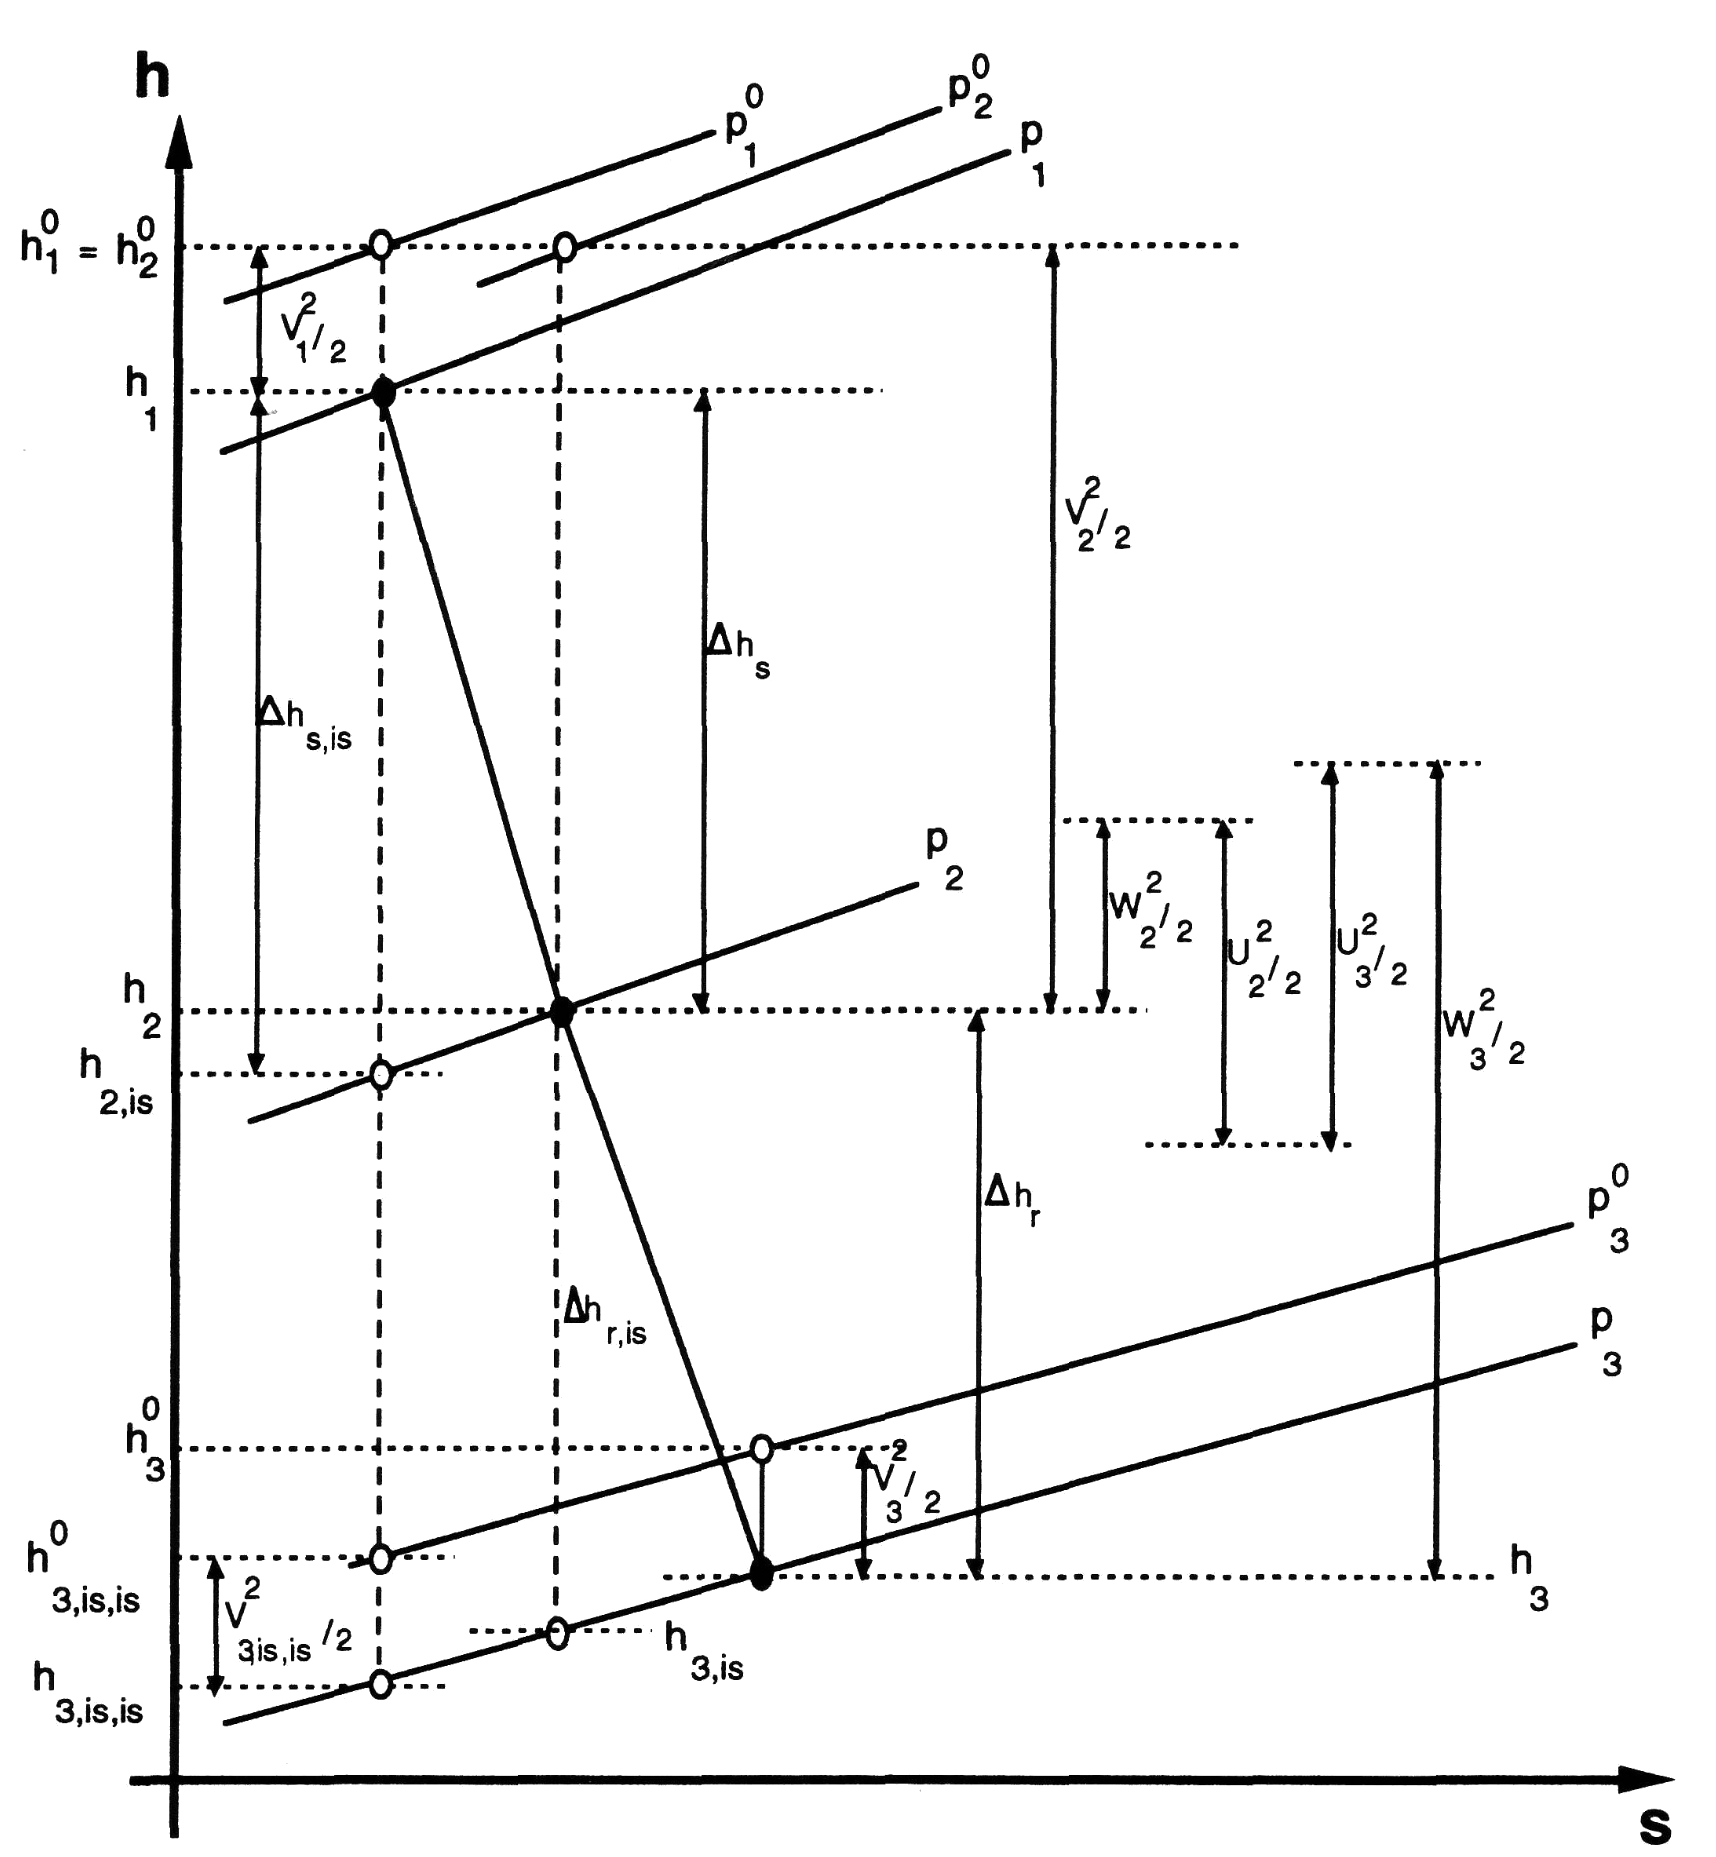
\includegraphics[width=0.5\textwidth]{Turb_mollier.png}
\caption{Mollier diagram of a turbine stage \citep{Hillewaert2019}}
\label{fig:C3_Mollierturb}
\end{figure}

\subsubsection{Axial turbine design and degree of reaction}
\quad\, The last written paragraph mentioned that some turbine are designed to put all the pressure drop over the stator to limit the axial force generated in the rotor.

It is possible to classify the turbines by creating two categories based on the degree of reaction $R$. The degree of reaction is defined as being the ratio between the static enthalpy drop over the rotor and the static enthalpy drop over the turbine stage.
\begin{equation}
R = \frac{h_2 - h_3}{h_1 - h_3}\label{eq:C3_R}
\end{equation}
Then the two families are 

\begin{itemize}
\setstretch{1}
\item The impulse or action turbines: The degree of reaction $R\simeq 0$. Thus, since the rotor doesn't see any pressure difference, the axial thrust on the shaft is minimized. The impulse turbines are often used for high pressure turbines (due to their small aspect ratio).
\item The reaction turbines: The degree of reaction $R$ is often between 0.5 and 0.7. This means that the pressure drop is distributed between the stator and the rotor. 
\end{itemize}

\subsubsection{Performance maps}
\quad\, The turbines can be also be characterized by a performance map determined from experimental results. The map is often composed of two performance plots as shown on Figure \ref{fig:C3_turbmap}.

\begin{figure}[h]
\centering
\includegraphics[width=\textwidth]{Turb_Map.png}
\caption{Illustration of a turbine performance map}
\label{fig:C3_turbmap}
\end{figure}  

The two plots on the Figure \ref{fig:C3_turbmap} illustrates for each iso-rotational speed $N_t$ the relationships $\Pi_t(\dot{m}_c,N_t)$ and $\eta_t(\dot{m}_c,N_t)$. As it can be noticed on the left diagram, all the curves tends to reach the same asymptotic values as the mass flow rate increases. This is due to the choking phenomena that limits at some point the flow rate through the compressor.\\

In this section about turbomachines, the most important notions for the good understanding of the future development have been given. Particularly, the concept of performance maps has been introduced, and a method of extrapolation using the similarity have been provided. 

Also, the descriptions of the compression and the expansion have been explained using the hs Mollier diagrams. Those diagrams, along with the schematic of the compressor and turbine stages, allows to describes with a decent accuracy the two previously mentioned transformation. 
\newpage
\newpage
\input{Chapter_3_-_Thermodynamic_components/Combustion_Chamber.tex}
\newpage
\section{Heat exchangers}
\quad\, The last important component that has to be defined and characterized is the heat-exchanger (HX). As the name says, the purpose of this element is to transfer the heat from a \textbf{hot} fluid to a \textbf{cold} fluid. The heat-exchangers can be classified into several categories\citep{Ngendakumana2018}.

\begin{itemize}
\setstretch{1}
\item The recuperators: their purpose is to recover the heat from a hot fluid to heat up a cold fluid for direct usage. For instance, the exhaust gas from a boiler will go through a recuperator to exchange its energy with water. For this application and for many others, the two streams within the HX are separated by physical walls.

Alternatively, the heat exchange can be performance by direct contact between the two fluids. In this case, nothing prevents the hot flow to mix with the cold flow (and vice versa).
\item The regenerators: considering a cycle , the purpose of the regenerators is to use a hot flow from the cycle to heat up a cold flow from the same cycle. 
\end{itemize}

By definition, the hot stream is the one that \textbf{provides} the heat, and the cold stream is the one \textbf{receiving} the heat.

On the Figure \ref{fig:C3_HX} are illustrated some schematics of heat-exchanger owning at different families.
\begin{figure}[h]
\centering
\subfloat[HX with fined plates \citep{Ngendakumana2018}\label{fig:C3_HX_fin_plate}]{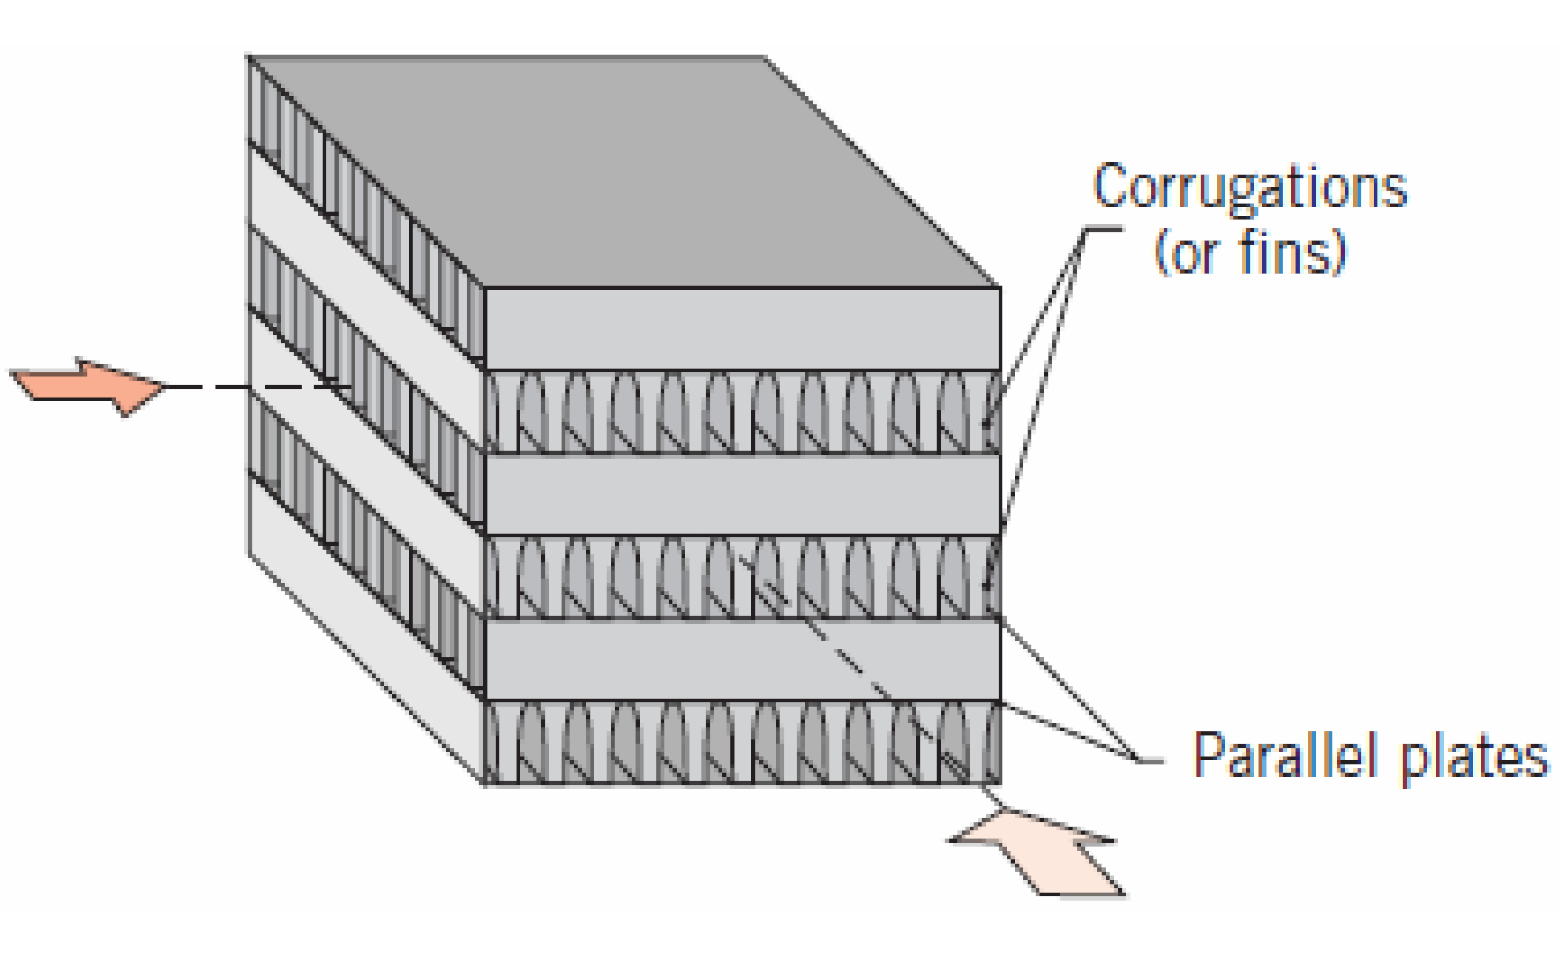
\includegraphics[width=0.4\textwidth]{HX_fin_plate}}\hfill
\subfloat[HX with fined tubes \citep{Ngendakumana2018}\label{fig:C3_HX_fin_tube}] {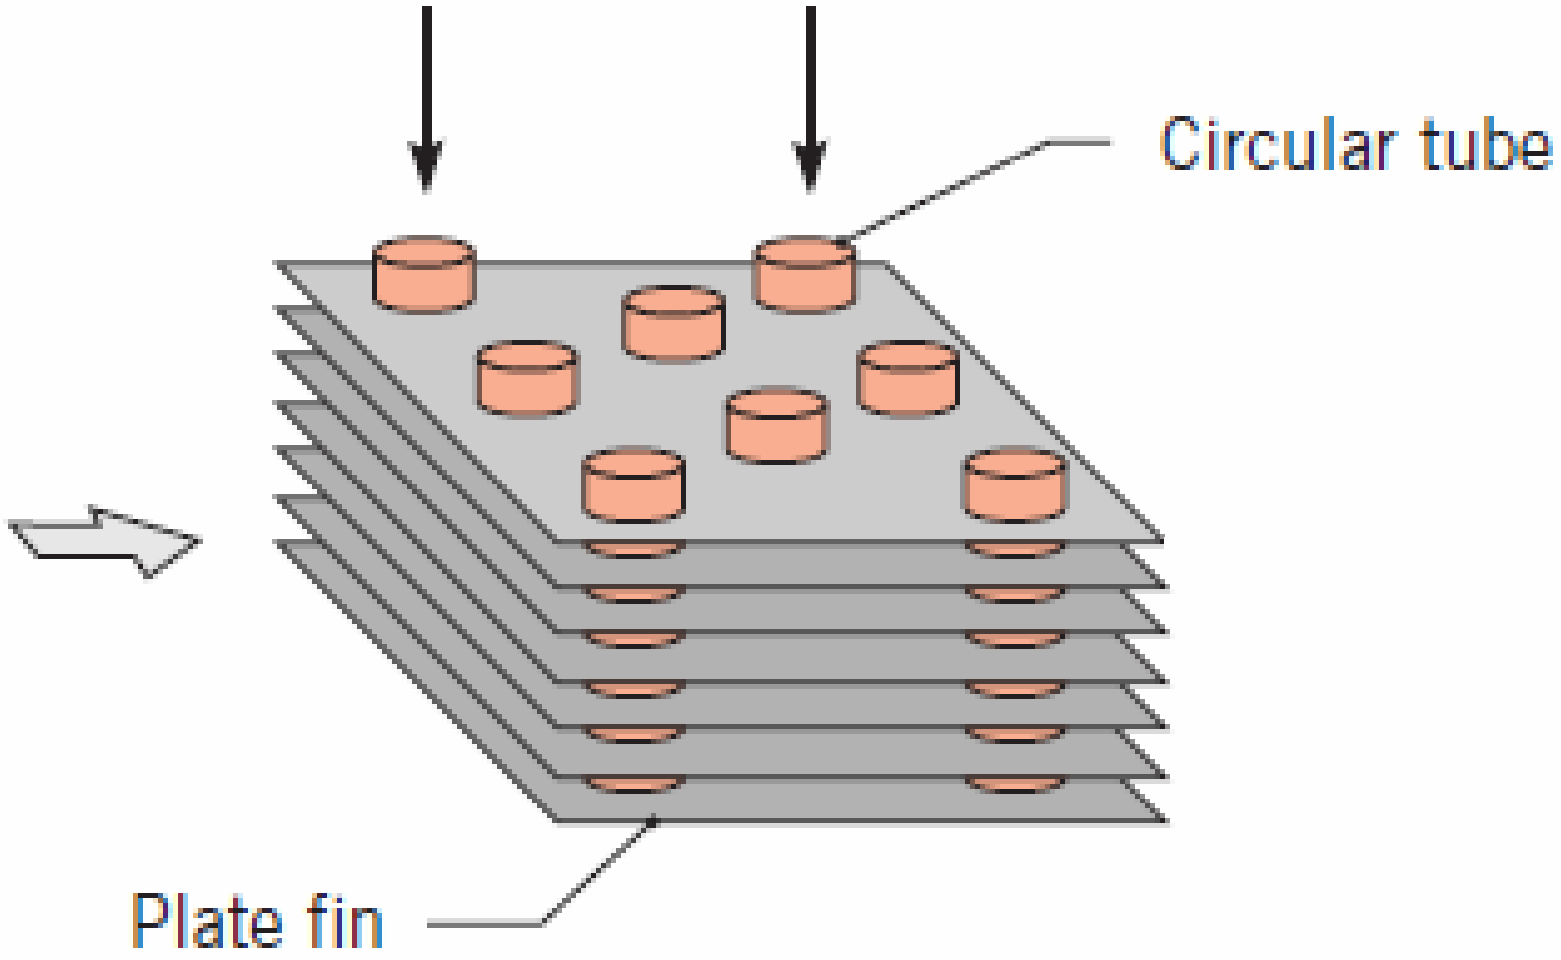
\includegraphics[width=0.4\textwidth]{HX_fin_tube}}\hfill
\subfloat[Plate heat exchangers \citep{Ngendakumana2018}\label{fig:C3_PHE}]{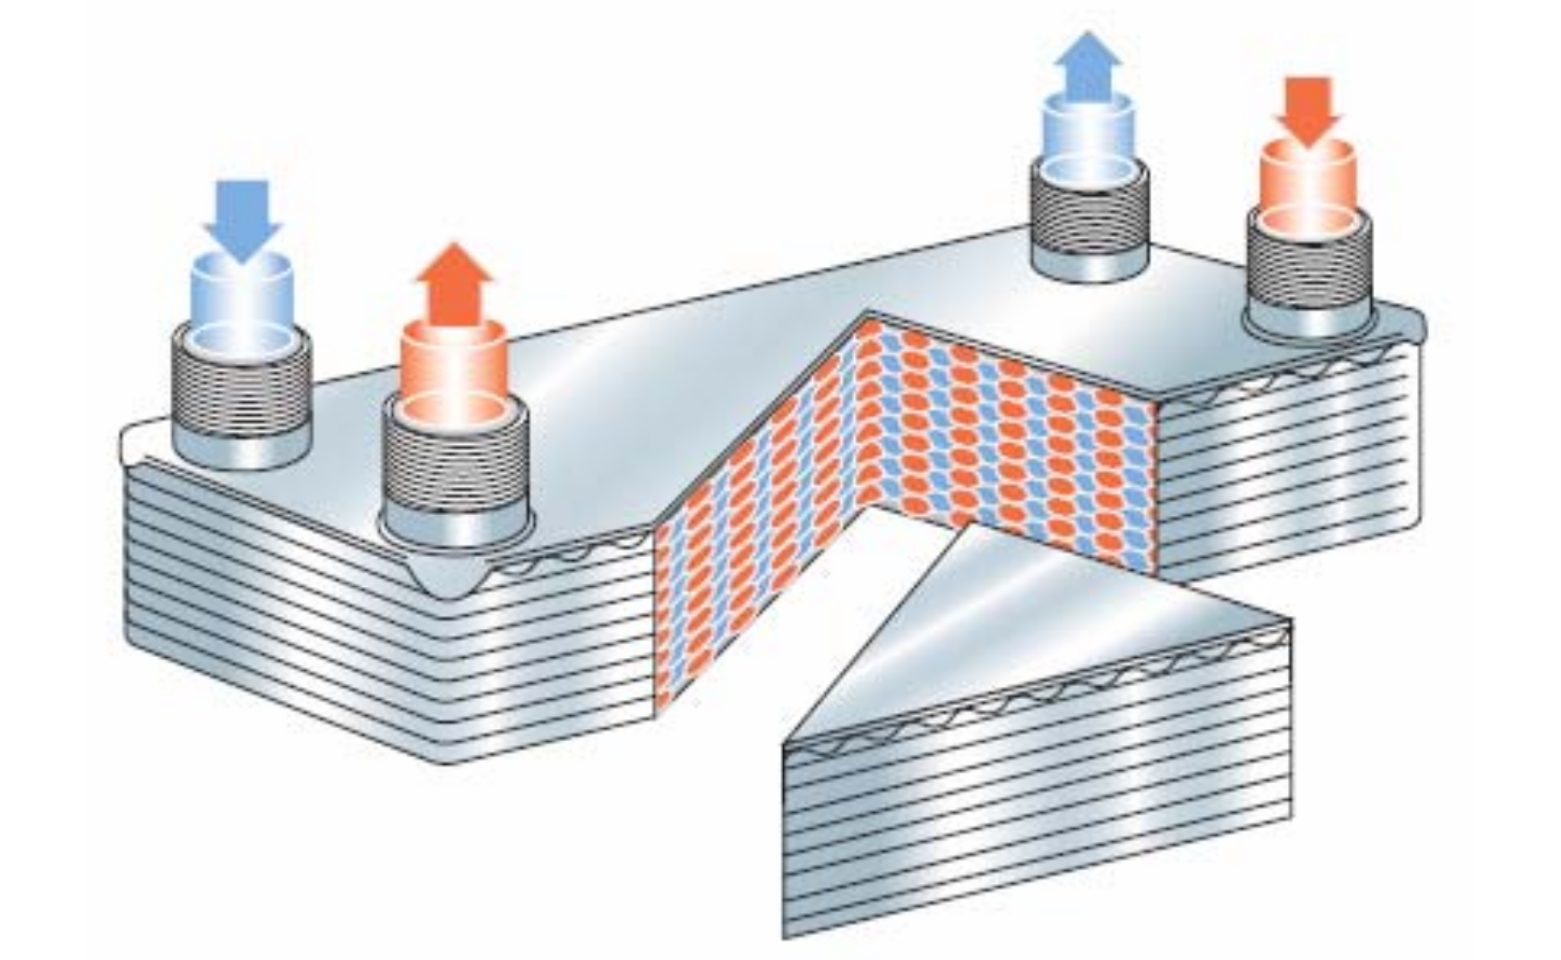
\includegraphics[width=0.4\textwidth]{HX_brased_plate}}
\caption{HX illustrations} \label{fig:C3_HX}
\end{figure}

The selected family will highly depends on the type of application that is targeted. Plate heat exchangers are one of the most compact type of heat exchangers. This compactness is highly appreciated for any system where the foot print and volume has to be as minimal as possible. However, this is at the cost of more complicated maintenance due the brazing of the plates.

This section will not cover the specificity of these different families. Instead, the main notions which are necessary to characterized the heat transfer between two fluids will be given.

\subsection{Stream configurations}
\quad\, There isn't an unique configuration regarding about the interaction between the hot and cold streams. Indeed, here are the main categories based on flow configurations.

\begin{itemize}
\setstretch{1}
\begin{figure}[h]
\centering
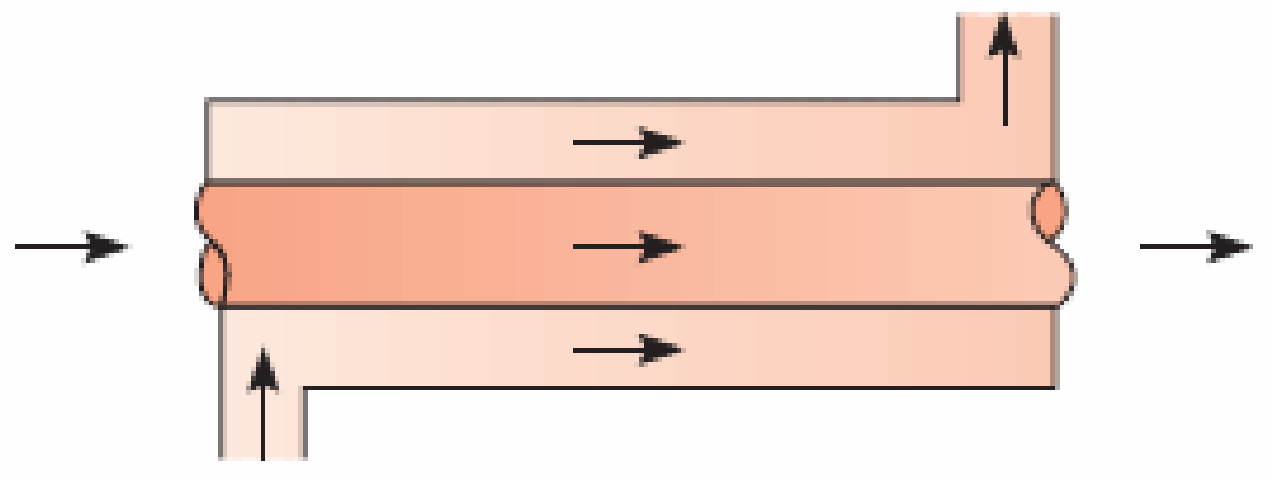
\includegraphics[width=0.4\textwidth]{parallele_flow}
\caption{Parallel flow heat exchanger \citep{Ngendakumana2018}}
\label{fig:C3_para_flow}
\end{figure}

\item Parallel flow HX: The two streams go through the heat exchanger in the same direction. 

\begin{figure}[h]
\centering
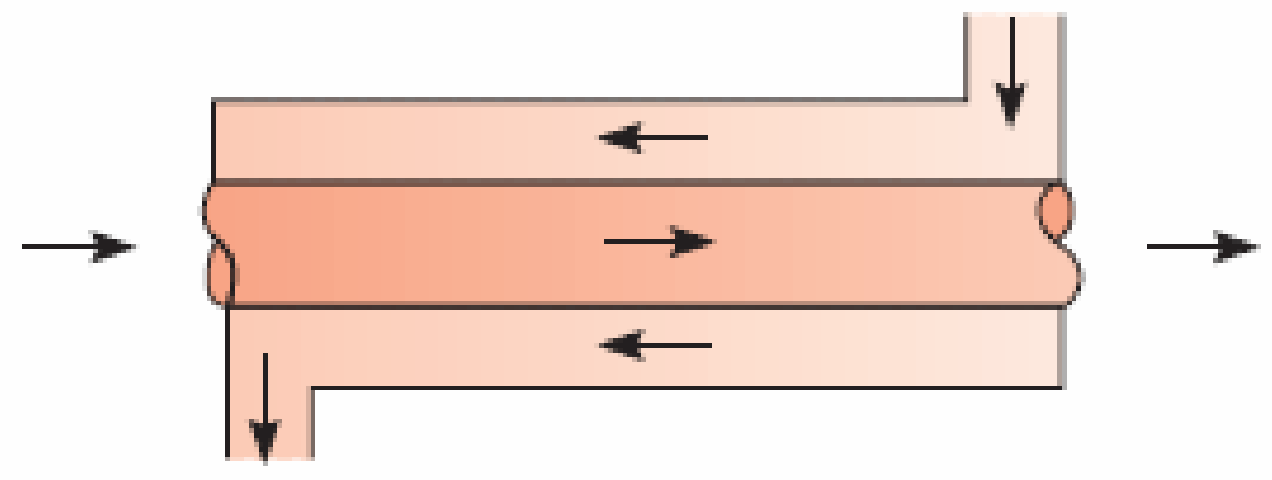
\includegraphics[width=0.4\textwidth]{opposite_flow}
\caption{Counter flow heat exchanger \citep{Ngendakumana2018}}
\label{fig:C3_counter_flow}
\end{figure}

\item Counter flow HX: The two streams go through the heat exchanger in the opposite direction. This configuration is more frequent than the parallel flow HX due to higher efficiency.

\begin{figure}[h]
\centering
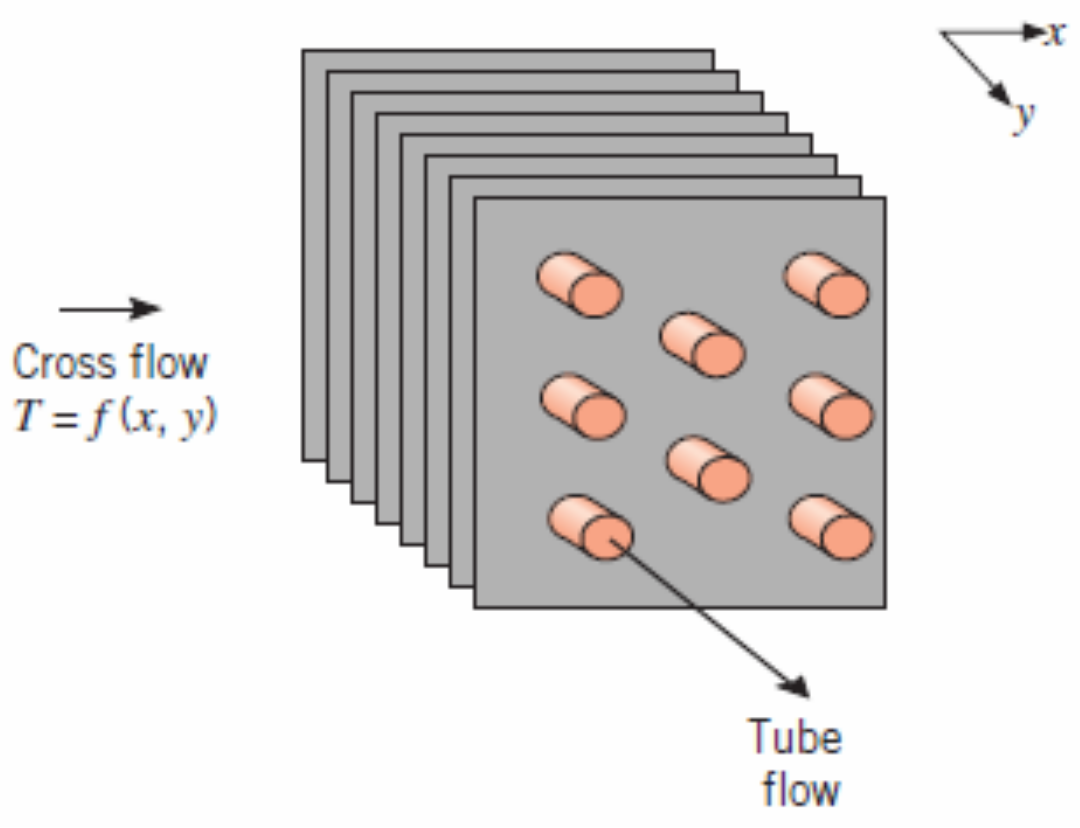
\includegraphics[width=0.4\textwidth]{crossed_flow_non_mixed}
\caption{Cross flow heat exchanger, both fluids unmixed \citep{Ngendakumana2018}}
\label{fig:C3_cross_flow_unmixed}
\end{figure}

\item Cross flow HX, both fluids unmixed: The flow in the tube does not sees the property of cross flow varying along with the distance traveled. Both flow are unmixed.
\newpage
\begin{figure}[h]
\centering
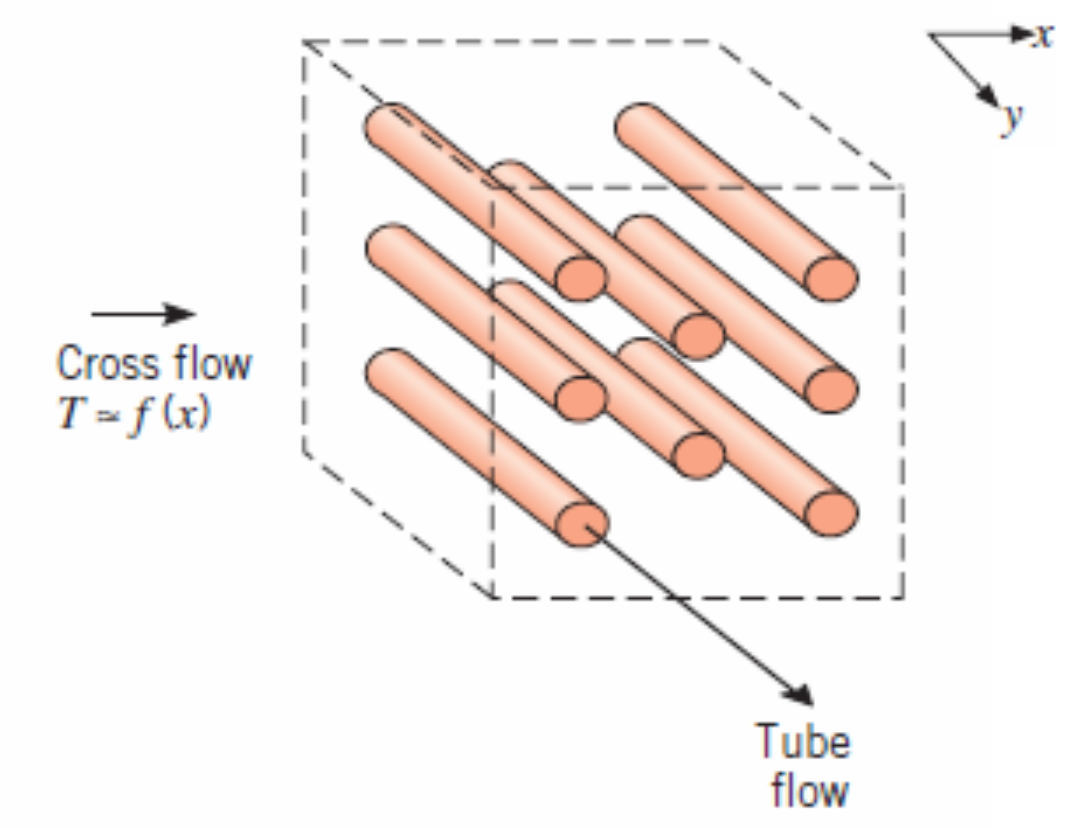
\includegraphics[width=0.4\textwidth]{crossed_flow_one_mixed}
\caption{Cross flow heat exchanger, one fluid mixed \citep{Ngendakumana2018}}
\label{fig:C3_cross_flow_1mixed}
\end{figure}

\item Cross flow HX, one fluid mixed: The flow in the tube does not sees the property of cross flow varying along with the distance traveled. The cross flow does not travel inside isolated channels.
\end{itemize}

Considering the parallel and counter flow heat exchanger, Two temperature differences can be defined based on the temperature profiles (Figure \ref{fig:C3_Tprof}) of both fluids inside the heat exchanger.

\begin{figure}[h]
\centering
\subfloat[Temperature profil for parallel flow HX \citep{Ngendakumana2018}\label{fig:C3_HX_par_flow_T}]{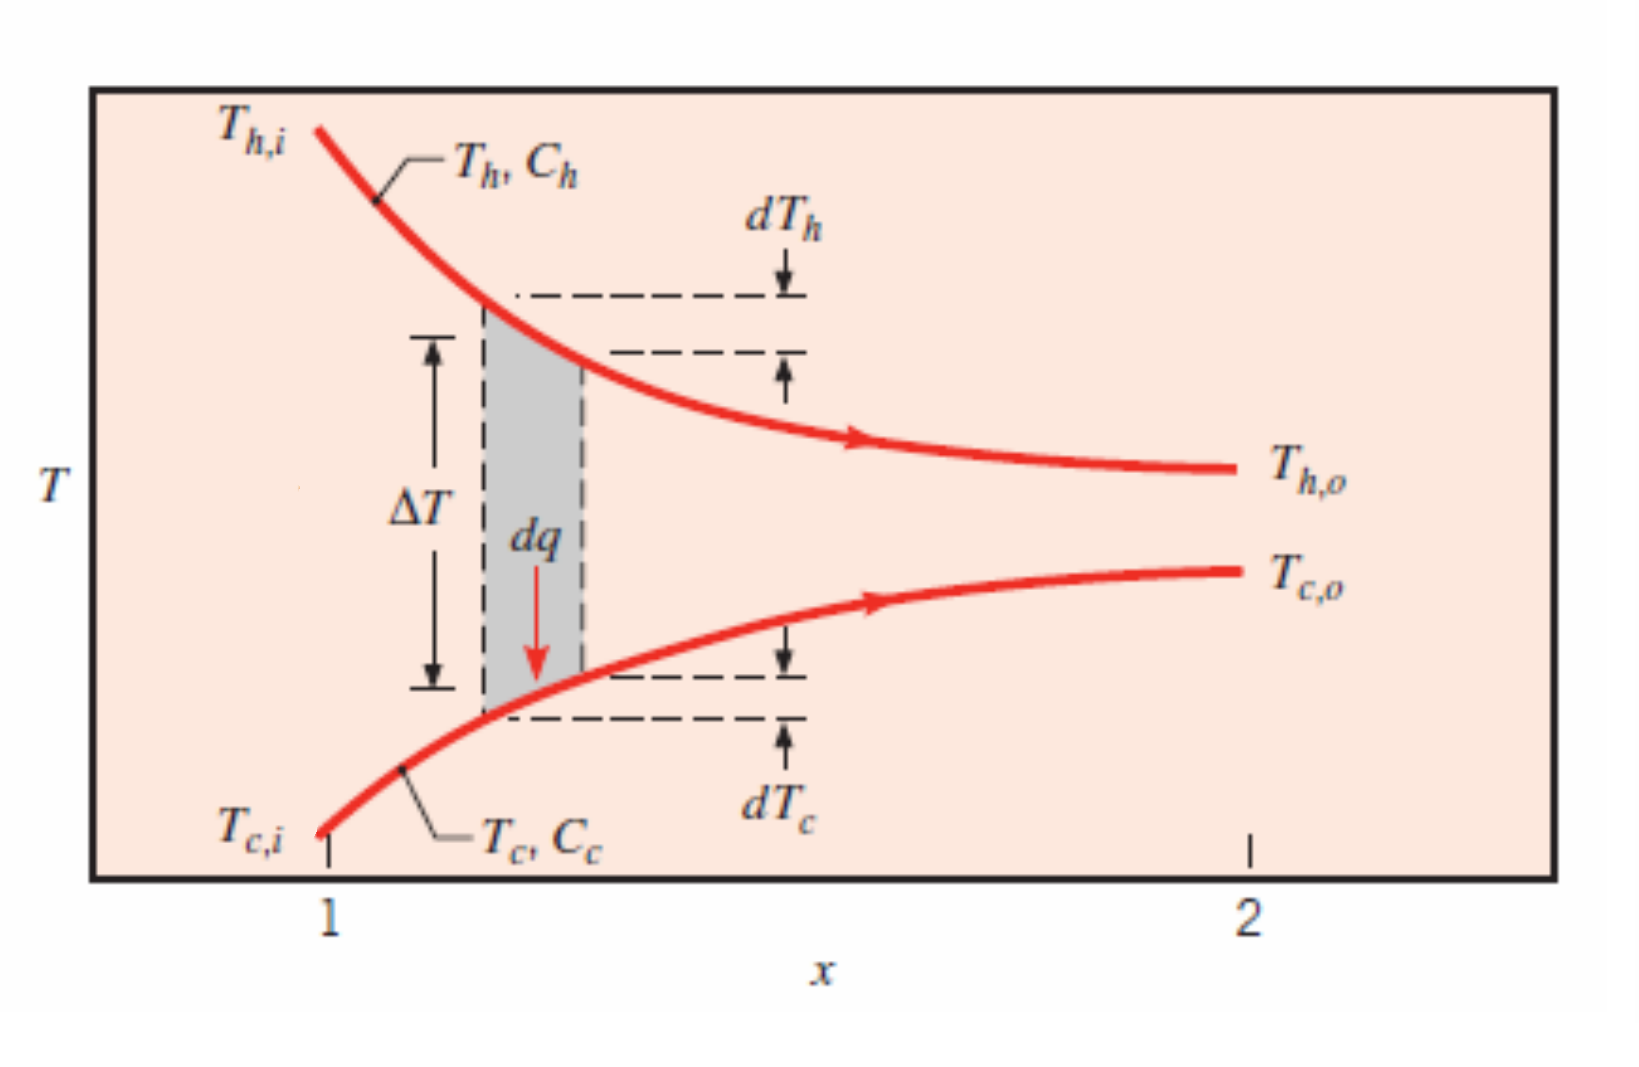
\includegraphics[width=0.45\textwidth]{parallele_flow_T}}\hfill
\subfloat[Temperature profil for counter flow HX \citep{Ngendakumana2018}\label{fig:C3_HX_opo_flow_T}] {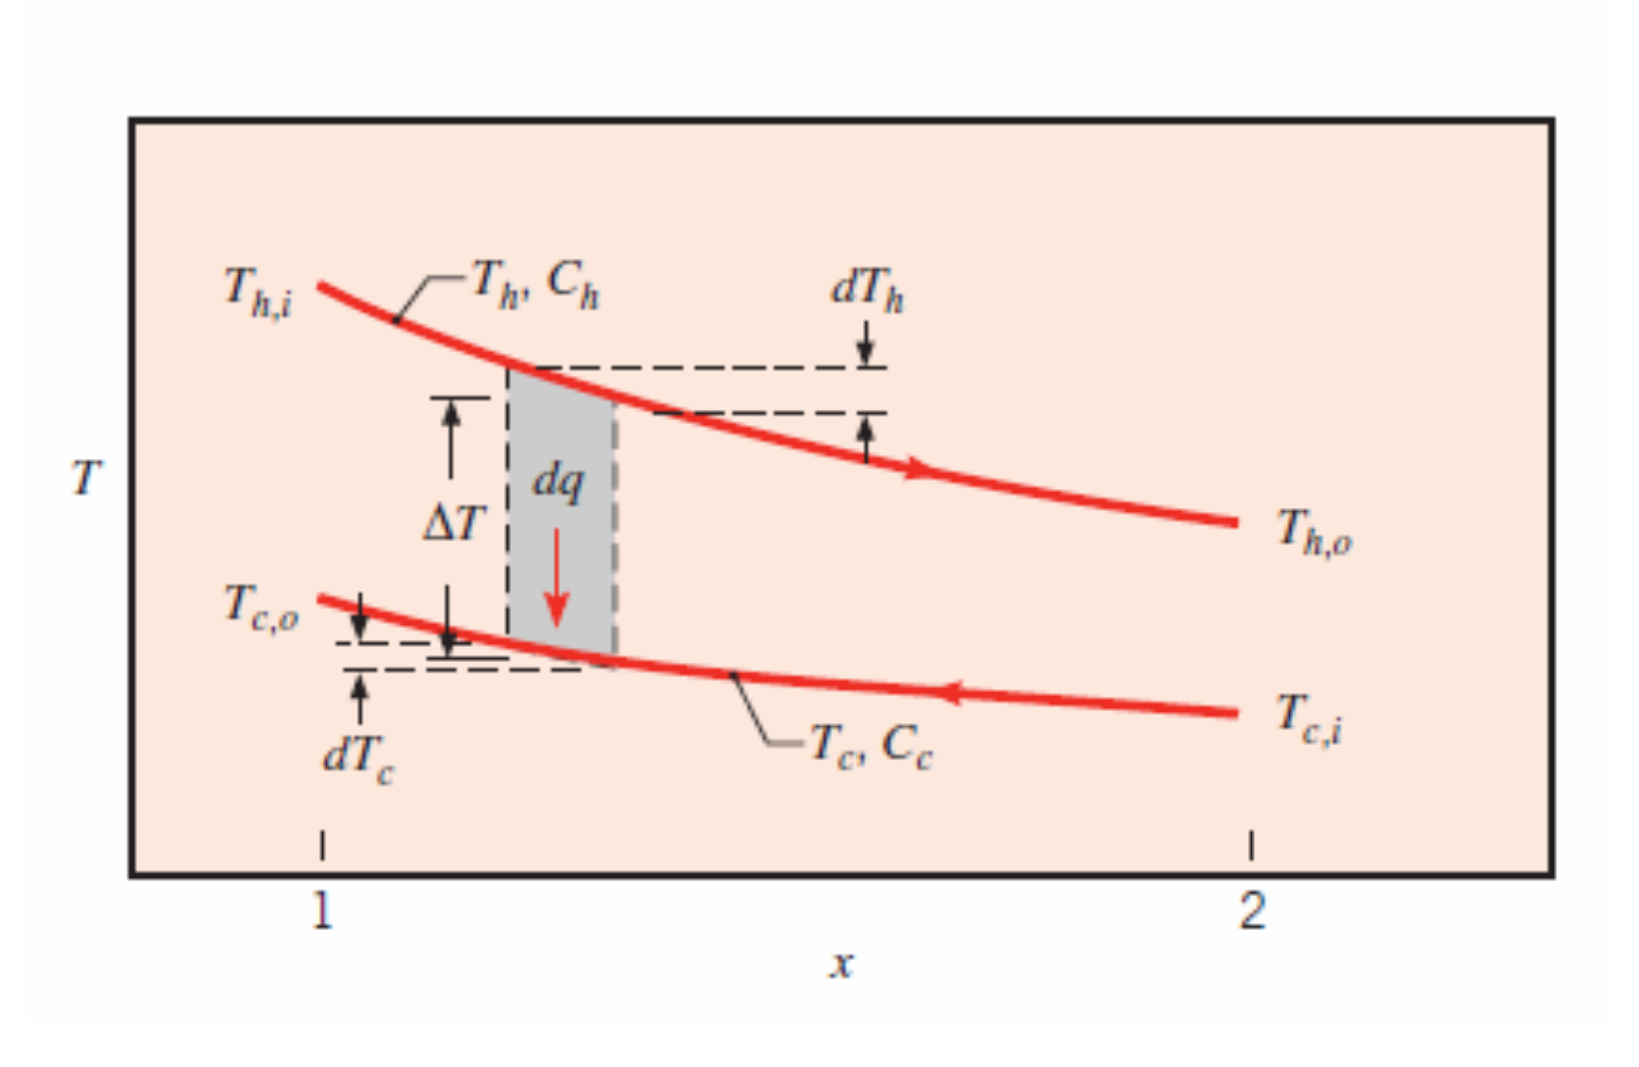
\includegraphics[width=0.45\textwidth]{opposite_flow_T}}\caption{Temperature profiles for different stream configurations}\label{fig:C3_Tprof}
\end{figure}

where the subscripts h and c indicate which flow is considered (h:hot; c:cold), and the subscripts i and o refer to the inlet and the outlet of the heat exchanger.

The first temperature difference $\Delta T_0$ is defined as being the largest temperature difference between the two flows, regardless the position inside the HX. Thus,

\begin{equation}
\setstretch{1}
\Delta T_0 =
\begin{cases}
T_{h,i} - T_{c,i} \text{ For the parallel flow}\\
T_{h,i} - T_{c,o} \text{ For the counter flow}\\
\end{cases}\label{eq:C3_DT0}
\end{equation}

The second temperature difference $\Delta T_L$ corresponds to the smallest temperature difference between the two flows. Thus,
\begin{equation}
\setstretch{1}
\Delta T_0 =
\begin{cases}
T_{h,o} - T_{c,o} \text{ For the parallel flow}\\
T_{h,o} - T_{c,i} \text{ For the counter flow}\\
\end{cases}\label{eq:C3_DTL}
\end{equation}

\subsection{Heat transfer within a heat-exchanger}
\quad\, The heat transfer rate of a heat exchanger is directly dependent on the nature of the fluids and the heat-exchanger itself. Let's consider the following relation (\ref{eq:C3_Qdot1})
\begin{equation}
\dot{Q} = \frac{\Delta T_{LM}}{R}= A\cdot U\cdot \Delta T_{LM}\text{ ( in W)}\label{eq:C3_Qdot1}
\end{equation}
where $A$ is the global surface area of the HX, and $R$ and $U$ are the global thermal resistance and transfer coefficient respectively. The $\Delta T_{LM}$ is called the logarithmic mean temperature difference. It's definition is
\begin{equation}
\Delta T_{LM} = \frac{\Delta T_0-\Delta T_L}{ln\left(\frac{\Delta T_0}{\Delta T_L}\right)}\label{eq:C3_lmtd}
\end{equation} 
with $ln$ being the neperian logarithm.
\subsubsection{Transfer coefficient}
The general definition for the product $A\cdot U$ is 
\begin{equation}
\frac{1}{A\cdot U}  = \frac{1}{\eta_{0,c}\cdot h_c \cdot A_c} + \frac{F_c}{\eta_{0,c}\cdot A_c} + R_w + \frac{F_h}{\eta_{0,h}\cdot A_h} + \frac{1}{\eta_{0,h}\cdot h_h \cdot A_h}\label{eq:C3_AU}
\end{equation}
where $h$ is the convective heat transfer coefficient (in W/m$^2$/K) of the fluid, $F$ is a degradation factor due to the clogging, $\eta_0$ is the global efficiency of the surface and $R_w$ is the wall resistance. 

It can be shown that the convective heat transfer coefficient $h$ is proportional to $\dot{m}^{4/5}$ for a turbulent stream in a smooth duct. Turbulent stream are stream for which the heat transfer coefficient is the much higher thanks to a large disorder within the flow. This type of flow is reached when the Reynolds number $Re$ exceeds a certain value. In circular tubes this critical value is around 10000.
\begin{align}
&Re = \frac{\rho\cdot v\cdot D_h}{\mu}\\
\text{ with $D_h = \frac{4\cdot A_c}{P_c}$}& \text{ and $u=\frac{\dot{m}}{\rho\cdot\pi\cdot\frac{D_h^2}{4}}$}
\end{align}
where $\mu$ is the static viscosity of the fluid, $A_c$ and $P_c$ are the area and the perimeter of the surface crossed by the flow, $D_h$ is the hydraulic diameter and $v$ is the velocity in the pipe.

In the present work, the heat exchanger that will be used are plate heat exchangers. For this specific category, the surface $A$ for the cold and the hot side are very closed from each others. Also, if the flow considered is only composed of one phase (i.e. only liquid or gaseous), the wall resistance $R_w$ can be neglected. 

If the efficiency $\eta$ are supposed equal for both the hot and the cold side and if the degradation factors $F$ are neglected, then the product $A\cdot U$ is proportional to
\begin{equation}
A\cdot U \div \frac{\dot{m}_h^{4/5}\cdot\dot{m}_c^{4/5}}{\dot{m}_h^{4/5} + \dot{m}_c^{4/5}}\label{eq:C3_AU_prop}
\end{equation}
\subsubsection{LMTD method}
\quad\, In the previous lines, a definition of the heat transfer rate based on the global transfer coefficient. This method is called the LMTD method and requires the knowledge of the geometry of the heat exchanger.
When the $\dot{Q}$ has been calculated, the temperatures at the outlet of the heat exchanger for the cold and hot stream can be computed using the two equations (\ref{eq:C3_ThQ}) and (\ref{eq:C3_TcQ}).
\begin{subequations}
\setstretch{1}
\begin{equation}
\dot{Q} = \dot{m}_h\cdot c_{p,h}\cdot(T_{h,in} - T_{h,out}) =\dot{C}_h\cdot(T_{h,in} - T_{h,out}) \label{eq:C3_ThQ}
\end{equation}
\begin{equation}
\dot{Q} = \dot{m}_c\cdot c_{p,c}\cdot (T_{c,out} - T_{c,in}) =\dot{C}_c\cdot (T_{c,out} - T_{c,in}) \label{eq:C3_TcQ} 
\end{equation}
\end{subequations}

This method requires the knowledge of the inlet and outlet temperatures of both fluids before initiating the computation of the heat transfer rate $\dot{Q}$ using the relation (\ref{eq:C3_Qdot1}). Therefore, this method needs iteration in the event where these temperatures are not known a priori.

\subsubsection{$\varepsilon$-NTU method}
\quad\, There exists a second method for the evaluation of the heat transfer rate which does not need the outlet temperature of the fluids. First, the maximum heat transfer rate $\dot{Q}_{max}$ is computed.
\begin{equation}
\dot{Q}_{max} = \dot{C}_{min}\cdot (T_{h,in} - T_{c,in})
\end{equation}
with $\dot{C}_{min}=min(\dot{C}_h,\dot{C}_c)$
Then the heat transfer rate is equal to 
\begin{equation}
\dot{Q} = \varepsilon\cdot\dot{Q}_{max}
\end{equation}
where $\varepsilon$ is the efficiency of the heat exchanger. This efficiency is a function of the ratio $C_r = \frac{\dot{C}_{min}}{\dot{C}_{max}}$, the flow arrangement, and the number of transfer unit NTU defined as being the ratio
\begin{equation}
\text{NTU} = \frac{A\cdot U}{\dot{C}_{min}}\label{eq:C3_NTU}
\end{equation}

As said, the relations $\varepsilon(\text{NTU},C_r)$ and $\text{NTU}(\varepsilon,C_r)$ depend on the heat exchanger configurations. An non exhaustive list is written in the annex \ref{annex_epsNTU}\citep{GregoryNellis2015} 
%%%%%%%%%%%%%%%
%ECRIRE ANNEXE%
%%%%%%%%%%%%%%%

Once the coefficient $\varepsilon$ computed, the outlet temperatures of the fluids can be obtained using the relations (\ref{eq:C3_ThQ}) and (\ref{eq:C3_TcQ}).

\subsubsection{Rating and sizing problem}
\quad\, The $\varepsilon$-NTU method is really useful for solving rating and sizing problems.

On one hand, rating problem are problem that, based on the knowledge of the geometry of the heat exchanger, evaluates its performance for given inlet temperature for both fluids. For this kind of problem, the NTU is first computed. Then, the efficiency $\varepsilon$ is derived to allow the calculation of the heat transfer rate.

On the other hand, sizing problems are used for the design of heat exchanger to provide the wished outlet temperatures. There, the efficiency is first calculated and then the NTU is deduced. Finally, from the equation (\ref{eq:C3_NTU}) the heat transfer area $A$ can be obtained\citep{Ngendakumana2018}.

A mix of these two types of problems will be used during this work. Indeed, the efficiency $\varepsilon$ of the heat exchangers in the system are known for a certain nominal flow rate.    The knowledge of the nominal efficiency provides the required tools to compute the product $A\cdot U_{nom}$ using the sizing problem methodology. 

Then, based on the approximation (\ref{eq:C3_AU_prop}), the $U$ for the given condition can be obtained since the heat transfer area $A$ remains unchanged. Finally, the non nominal $U$ can be used to compute the non nominal efficiency $\varepsilon$ using rating problem.
\section{Piping and pressure drop}
\quad\, From now, the loss of pressure inside the different elements has not be considered. However, for a system like a gas turbine, the pressure drops have to be as minimal as possible to guaranty that the expanded gas in the turbine is at a pressure as high as possible. 

In this work, simple formula will be applied for the pressure drops computation. These one will be computed based on a pressure drop factor $Dp$ varying from 0 to 1. Then the pressure at the outlet of the component is given by
\begin{equation}
p_{o} = p_{i}\cdot (1 - Dp)
\end{equation}
where the factor $Dp$ is different for each component of the system. 

Before the present work, the pressure drop factors have been evaluated using computational fluid dynamics (CFD) for a nominal point of operation. Then, it can be demonstrated that the pressure difference $\Delta p = p_{i} - p_{o}$ is a quadratic function of the mass flow rate $\dot{m}$. Thus, the pressure losses for any non nominal points of operation are given by
\begin{equation}
\Delta p \simeq \Delta p_{nom}\cdot \frac{\dot{m}^2}{\dot{m}^2_{nom}}
\end{equation}

 %The following subsection will provide qualitative information about heat exchangers. The different families of HX based on the stream configurations or the geometries will be defined.
%
%\subsection{Families of heat exchangers}
%\quad\, Before studying the performances of any heat exchangers, it is interesting to establish a short state of the art. As it has been previously mentioned, among the heat exchangers can be distinguished the recuperators and the regenerators. However, these categories is based on the type of applications.
%
%\subsubsection{Families based on stream configurations}
%First, a categorization can be made based on the flow configurations within the heat exchanger. From this analysis, four can be created.
%
%\begin{itemize}
%\setstretch{1}
%\item Parallel flow HX: The two streams go through the heat exchanger in the same direction. 
%
%\begin{figure}[h]
%\centering
%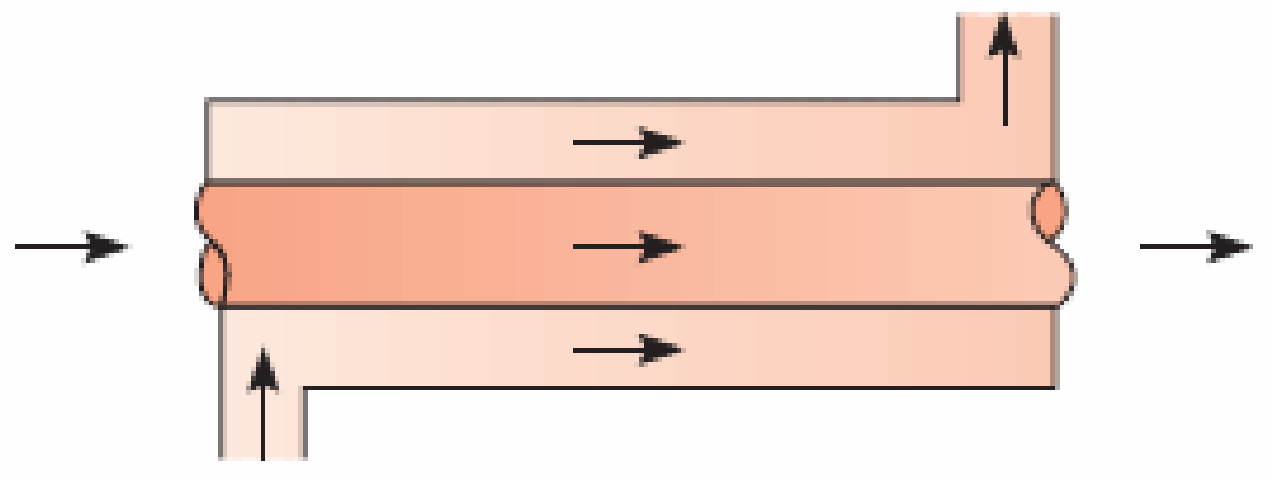
\includegraphics[width=0.5\textwidth]{parallele_flow}
%\caption{Parallel flow heat exchanger\citep{Ngendakumana2018}}
%\label{fig:C3_para_flow}
%\end{figure}
%\newpage
%\item Counter flow HX: The two streams go through the heat exchanger in the opposite direction. This configuration is more frequent than the parallel flow HX due to higher efficiency.
%\begin{figure}[h]
%\centering
%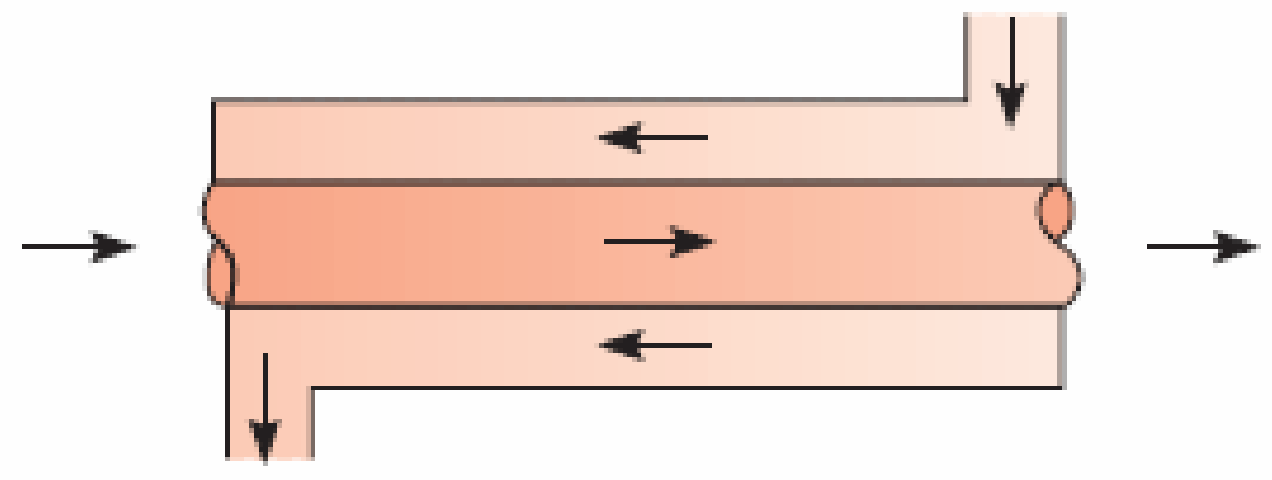
\includegraphics[width=0.5\textwidth]{opposite_flow}
%\caption{Counter flow heat exchanger\citep{Ngendakumana2018}}
%\label{fig:C3_counter_flow}
%\end{figure}
%
%\item Cross flow HX, both fluids unmixed:  This configuration, illustrated on Figure \ref{fig:C3_cross_flow_unmixed}. The flow in the tube does not sees the property of cross flow varying along with the distance traveled. Both flow are unmixed.
%\begin{figure}[h]
%\centering
%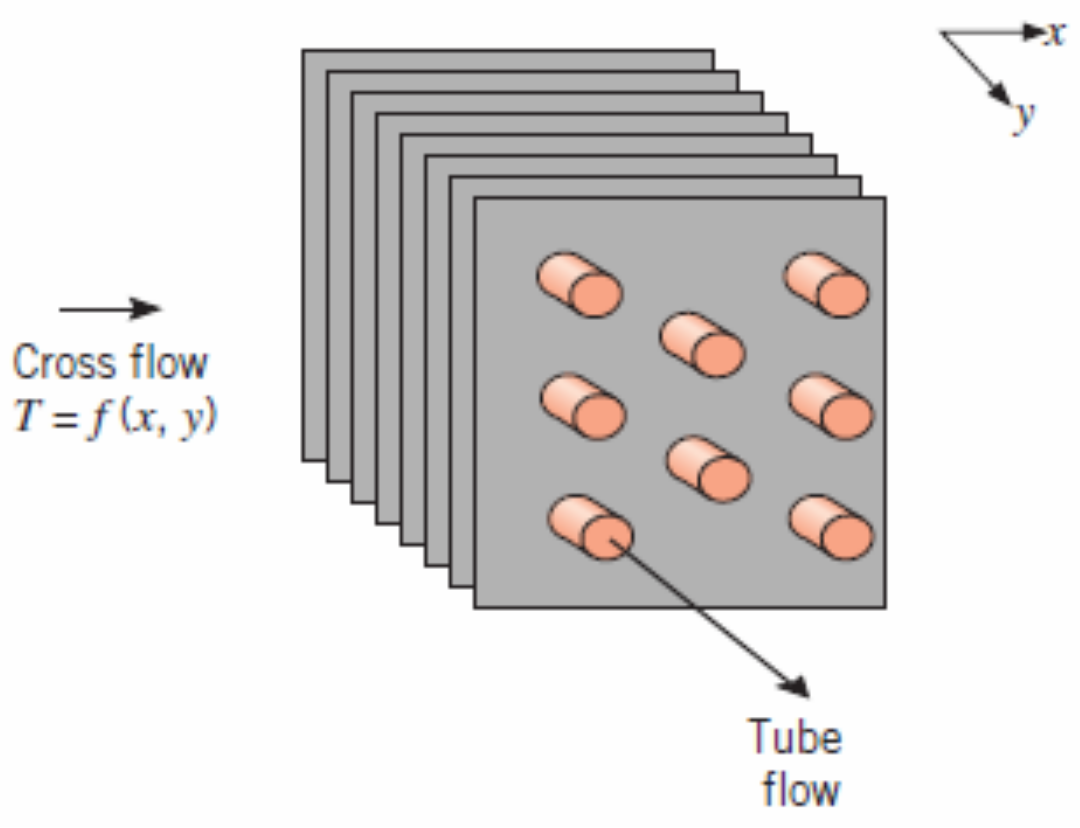
\includegraphics[width=0.4\textwidth]{crossed_flow_non_mixed}
%\caption{Cross flow heat exchanger, both fluids unmixed\citep{Ngendakumana2018}}
%\label{fig:C3_cross_flow_unmixed}
%\end{figure}
%\item Cross flow HX, one fluid mixed:  This configuration, illustrated on Figure \ref{fig:C3_cross_flow_1mixed}. The flow in the tube does not sees the property of cross flow varying along with the distance traveled. The cross flow does not travel inside isolated channels.
%\begin{figure}[h]
%\centering
%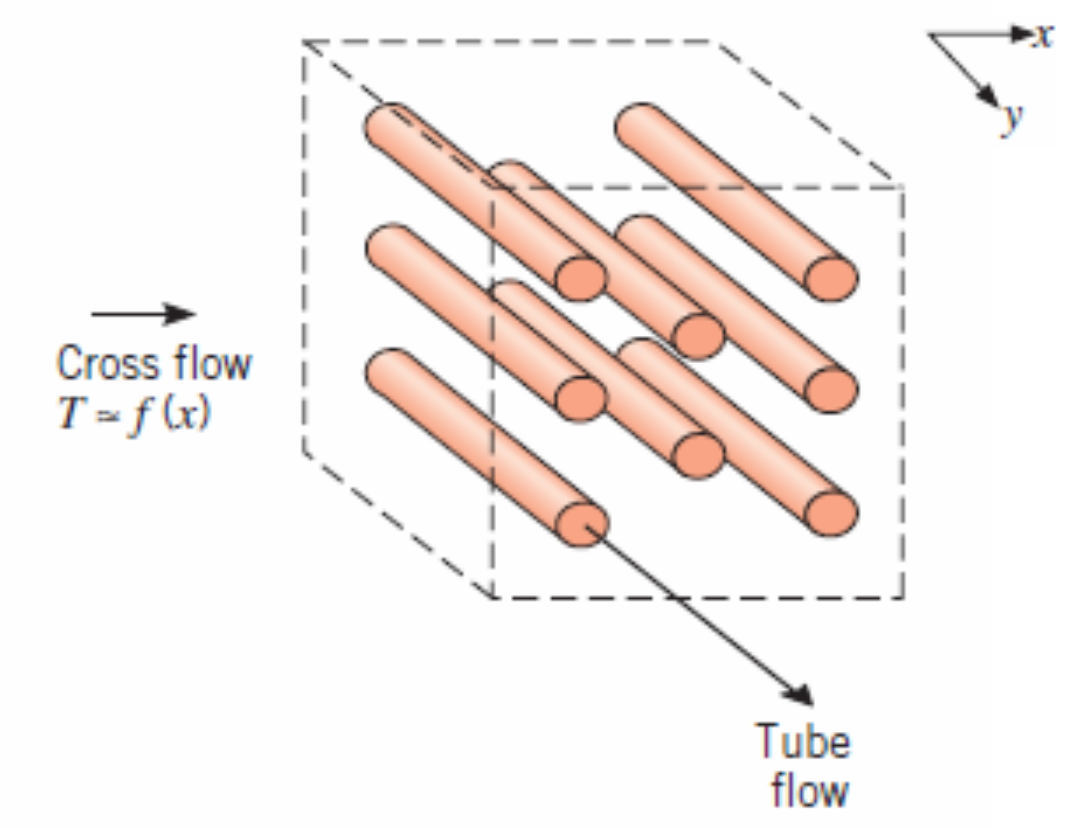
\includegraphics[width=0.4\textwidth]{crossed_flow_one_mixed}
%\caption{Cross flow heat exchanger, one fluid mixed\citep{Ngendakumana2018}}
%\label{fig:C3_cross_flow_1mixed}
%\end{figure}
%\end{itemize}
%
%\subsubsection{Families based on the HX construction}




% \section{Notion about Thermodynamics}


% % Introduire les différentes notions de base qui seront utiles pour la suites.
% % - Enthalpy
% % - Entropy
% % - H-s diagram
% % - Heat transfer
% \section{Description of the Brayton cycle}
% % "A thermodynamic cycle consists of a linked sequence of thermodynamic processes that involve transfer of heat and work into and out of the system, while varying pressure, temperature, and other state variables within the system, and that eventually returns the system to its initial state. In the process of passing through a cycle, the working fluid (system) may convert heat from a warm source into useful work, and dispose of the remaining heat to a cold sink, thereby acting as a heat engine. Conversely, the cycle may be reversed and use work to move heat from a cold source and transfer it to a warm sink thereby acting as a heat pump. At every point in the cycle, the system is in thermodynamic equilibrium, so the cycle is reversible (its entropy change is zero, as entropy is a state function)."
% % 
% \section{What is the Brayton cycle?}
% \subsection{presentation of the cycle}
% \subsection{Why is it called thermodynamic cycle?}
% \section{Theoretical notions about thermodynamic}
% \subsection{What is the enthalpy?}
% \subsection{Why using the enthalpy for thermodynamic state assessment?}
% \subsection{What is the entropy?}
% \section{Description of the compressor}
% \subsection{What is a compressor?}
% \subsection{Modelling - outlet enthalpy calculation}
% \section{Description of the turbine}
% \subsection{What is a turbine?}
% \subsection{Modelling - outlet enthalpy calculation}
% \section{Description of the combustion chamber}
% \subsection{What is a combustion chamber?}
% \subsection{Modelling - Combustion equation using mass conservation} 
% \section{Description of the heat-exchanger}
% \subsection{What is a heat-exchanger?}
% \subsection{Modelling - Pinch temperature method}
% \subsection{Modelling - epsilon-NTU method}
% \section{Description of the piping}
% \subsection{Modelling of the pressure drop (correlation)}	
% \section{Analysis of the possible configuration for the Brayton cycle}
% \chapter{Brayton cycle – Python implementation}
% \section{What is Python and why using it as programming language?}
% \section{Structure of the Python code}
% \subsection{Module description}
% \subsection{Improvement of the Python code}
% \chapter{Component performance map integration}
% \section{What is a performance map?}
% \section{What is the interest of using performance maps?} 	
% \subsection{For the turbomachines}
% \subsection{For the heat-exchangers}
% \subsection{For the piping}
% \subsection{For the combustion chamber}
% \section{Build of the map using least squares fitting}
% \subsection{Data used}
% \subsection{Interpolation scheme}
% \section{Quality of the interpolation}
% \subsection{Error on the sample values}
% \subsection{Cost function}
% \chapter{Gas composition integration}
% \section{Why considering the gas composition?}
% \section{Fumes composition computation}
% \section{Thermodynamic state evaluation}
% \subsection{Use of the NASA table}
% \subsection{Comparison for fumes state computation (old vs new method)}
% \chapter{Experimental test bench}
% \section{Presentation of the different parts}
% \section{Analysis of the results}




% \quad\, In the introduction, the ideal Brayton cycle has been presented and analysed. Some improvements have been proposed to increase the efficiency of the system.\\
% 
% This chapter will be focused on the development of a deterministic model of the cycle using Python as the programming language. First will be given a overview of the structure of the program. Then, from a model already developed, some modifications will be provided to gain slightly

% \section{Overview of the cycle}
% \quad\, The cycle modelled will be composed of non ideal components and will include a regenerator followed by a recuperator for heated water production. A schematic is presented on Figure \ref{fig:schema_cycle}.

% % \begin{figure}[h!]
% %     \centering
% %     \includegraphics[width=0.8\textwidth]{Deterministic_modelling/schema_BC.png}
% %     \caption{Brayton cycle schematic. values are for nominal conditions}
% %     \label{fig:schema_cycle}
% % \end{figure}

% On the graph are emphasised the main steps of the cycle:
% \begin{itemize}
%     \item Compressor ($\mathbf{1} \Rightarrow\mathbf{2}$): The ambient air is compressed by the compressor to rise its pressure. 
%     \item Recuperator - \textit{cold side} ($\mathbf{2} \Rightarrow\mathbf{3}$): The air from the compressor is heated up by the hot gas from the turbine.
%     \item Combustion Chamber ($\mathbf{3} \Rightarrow\mathbf{4}$): Fuel is injected to create a combustion to increase the enthalpy of the gas. The mass flow of fuel injected is calculated based on the wished TIT. 
%     \item Turbine ($\mathbf{4} \Rightarrow\mathbf{5}$): The gas from the combustion chamber is expanded through the turbine. The produced power will be partly consumed by the compressor. The leftover is absorbed by the generator.
%     \item Regenerator - \textit{hot side} ($\mathbf{5} \Rightarrow\mathbf{6}$): The hot gas from the turbine are cooled down when going through the regenerator. 
%     \item Recuperator ($\mathbf{6} \Rightarrow\mathbf{7}$): The remaining heat is used to heat up water. The target temperature for the water depend on the need. The gas is then released to the atmosphere.
% \end{itemize}

% This segmentation of the cycle is useful to properly pose the problem and to verify if every elements are well included in the program. 

% Moreover, it allows to identify what are the different components that play a role in the cycle. This identification is useful to isolate a specific element to work on. 

% \section{Description of the deterministic model}
% \quad\, This part of the chapter is dedicated to the analysis of the Brayton cycle deterministic model. The analysis will be segmented into several section. 

% First, the structure of the program will be given. Then, the description of the specific parts of the code will be provided. This analysis will allow to identify the possible modifications that will improve the performance and accuracy of the model. 
% \subsection{Structure of the program}
% % \begin{figure}[h]
% %     \centering
% %     \input{Deterministic_modelling/schema1}
% %     \caption{Caption}
% %     \label{fig:my_label}
% % \end{figure}
% %%%%%%%%%%%%%%%%%%%%%%%
% %% Map interpolation %%
% %%%%%%%%%%%%%%%%%%%%%%%
% \section{Interpolation map}
% \subsection{Definition}
% \subsection{Description of the components that will be modelled using maps}
% \subsection{Interpolation scheme}
% \subsubsection{Polynomial used}
% \subsubsection{Optimisation program}
% \textsc{P}: subset of $\mathbb{R}^{n\times 3}$. \textit{n} is the number of operational points.\\
% \textsc{A}: subset of $\mathbb{N}^{m\times 2}$. \textit{m} is the number of term in the polynomial and its value is
% \begin{equation}
%     m = \frac{(d+1)(d+2)}{2}
% \end{equation}
% with \textit{d} the maximum degree of the polynomial.
% \begin{equation*}
% \begin{aligned}
% & \underset{a\in\mathbb{R}}{\text{minimize}}
% & &  \textbf{F} = \sum_{k\in\textsc{P}}\left[z_k - f(x_k, y_k) \right]^2 \\
% & \text{with}
% & & f(x, y) = \sum_{i=0}^{d}\sum_{j=0}^{d-i} a[i,j]\cdot x^i\cdot y^j \; \forall x, y\in\mathbb{R}
% \end{aligned}
% \end{equation*}
% minimising $\textbf{F}$ is similar to forcing all the partial derivatives with respect to the a[i,j] to be equal to zeros. thus, the condition
% \begin{equation}
%     2 \cdot \sum_{k\in\textsc{P}}\left[z_k - f(x_k, y_k)\right] \cdot x_k^i \cdot y_k^j = 0
% \end{equation}
% has to be satisfied for all $\{i,j\}\in\textsc{A}$.
% \subsection{extrapolation of the compressor map to the small rotational speed}
% at low rotational speed, the approximation of a incompressible fluid can be done --> used of the similarity
% \begin{align}
%     \dot{m}_2 &= \dot{m}_1 \cdot \frac{N_2}{N_1}\\
%     \Delta H_2 &= \Delta H_1 \cdot \left(\frac{\Omega_2}{\Omega_1}\right)^2 \label{Delta H}\\
%     \eta_2 &= \eta_1
% \end{align}
% where $\Delta H = H_{ex} - H_{su}$\\
% Let consider the following references:
% \begin{align}
%     T_{\textbf{0}} & = 293.15K\\
%     H_{\textbf{0}} & = Cp\cdot T_{\textbf{}} \text{ with $Cp = 1005$  J/(kg$\cdot$ K)}\\
%     R & = 287 \text{ J/(kg$\cdot$ K)}\\
%     \gamma &= \frac{Cp -R}{Cp}
% \end{align}
% To go from the operational point \textbf{1} to the similar operational point \textbf{2}, the following relations are used.\\
% First the computation of $\Delta H_1$ is done.
% \begin{align*}
%     \frac{T_{\textbf{1},ex,s}}{T_{\textbf{1},su}} &= \left(\frac{P_{\textbf{1},ex}}{P_{\textbf{1},su}}\right)^{\frac{\gamma-1}{\gamma}} = \Pi_{\textbf{1}}^{\frac{\gamma-1}{\gamma}}\\
%     T_{\textbf{1},ex} &= T_{\textbf{1},su} + \frac{T_{\textbf{1},ex,s} - T_{\textbf{1},su}}{\eta_1}\\
%     H_{\textbf{1}, ex} &= H_{\textbf{0}} + Cp\cdot (T_{\textbf{1},ex} - T_{\textbf{0}})\\
%     \Rightarrow \Delta H_1 &= H_{\textbf{1}, ex} - H_{\textbf{1}, su}
% \end{align*}
% Then, using the equality \ref{Delta H}, the $\Delta H_2$. Then, going backward the pressure ratio $\Pi_{\textbf{2}}$ can be computed.
% \subsection{delimitation of the compressor map}
% Compressor --> surge line and chock line.\\
% surge line: level set using the left extreme points from the data (for each rotational speed N)\\
% chock line: approximation by using the maximal flow rate from the data as the maximal admissible flow rate.\\
% bottom limit: Pratio = 1\\



% %%%%%%%%%%%%%%%%%%%%%%
% %% Fluid Properties %%
% %%%%%%%%%%%%%%%%%%%%%%
% \section{Computation of the fluid's composition}
% CoolProp --> NASA table
% \subsection{Combustion's equations}
% \begin{align*}
%     \dot{m}_{ex}\cdot y_{ex,O2} &= \dot{m}_a\cdot y_{a,O2} - 2\cdot\dot{w}_{CH4}\cdot MM_{O2}\\
%     \dot{m}_{ex}\cdot y_{ex,Ar} &= \dot{m}_a\cdot y_{a,Ar}\\
%     \dot{m}_{ex}\cdot y_{ex,H2O} &= \dot{m}_a\cdot  y_{a,H2O} + 2\cdot\dot{w}_{CH4}\cdot MM_{H2O}\\
%     \dot{m}_{ex}\cdot y_{CO2} &= \dot{m}_{a}\cdot y_{a,CO2} + \dot{m}_{f}\cdot y_{f, CO2}
%     + \dot{w}_{CH4}\cdot MM_{CO2}\\
%     \dot{m}_{ex}\cdot y_{N2} &= \dot{m}_{a}\cdot y_{a, N2} + \dot{m}_{f} \cdot y_{f,N2}
% \end{align*}
% where $\dot{w}_{CH4} = \dot{m}_{f}\cdot \frac{y_{f,CH4}}{MM_{CH4}}$
% \subsection{Thermodynamic property computation}
% Let's considered a fluid labelled \textit{X}. The set \textsc{E} is composed of the list of the different species present in the fluid.
% \subsubsection{Enthalpy}
% The enthalpy of \textit{X} is equal to 
% \begin{equation}
%     h_{x} = \sum_{i\in\textsc{E}}y_{x,i}\cdot h_{x,i} 
% \end{equation}
% where the $h_{x,E}$ are the individual enthalpy of each component $i\in\textsc{E}$ computed using CoolProp. 
% \subsubsection{Heat capacity}
% \begin{align}
%     cp_{x} &= \sum_{i\in\textsc{E}}y_{x,i}\cdot cp_{x,i}\\
%     cv_{x} &= \sum_{i\in\textsc{E}}y_{x,i}\cdot cv_{x,i}
% \end{align}
% \subsubsection{Density}
% \begin{equation}
% \rho_{x} = \left(\sum_{i\in\textsc{E}} \frac{y_{x,i}}{\rho_{x,i}}\right)^{-1}
% \end{equation}
% \subsubsection{Dynamic viscosity}
% Wike's method
% \begin{equation}
%     \mu_{x} = \sum_{i\in\textsc{E}} y_{x,i}\cdot \frac{\mu_{x,i}}{A_{x,i}}
% \end{equation}
% where the $A_{x,i}$ are given by the following formula
% \begin{equation}
%     A_{x,i} = \sum_{j\in\textsc{E}} y_{x,j}\cdot \phi_{x,[i,j]}
% \end{equation}
% The $\phi_{x,[i,j]}$ being
% \begin{equation}
%     \phi_{x,[i,j]} = \frac{\left(1+\sqrt{\frac{\mu_{x,i}}{\mu_{x,j}}}\cdot\left(\frac{MM_{x,j}}{MM_{x,i}}\right)^ {0.25}\right)^2}{\sqrt{8\cdot\left(1+\frac{MM_{x,i}}{MM_{x,j}}\right)}}
% \end{equation}
% \section{Pressure drops computation}
% \subsection{friction coefficient in pipe}
% \begin{equation}
%     \mathit{Re} = \frac{V\cdot D\cdot \rho}{\mu}
% \end{equation}
% \begin{equation}
%     \frac{1}{\sqrt{f}} =  - 2\cdot \log\left(\frac{\varepsilon}{D\cdot 3.7} + \frac{2.51}{\mathit{Re}\cdot \sqrt{f}}\right)
% \end{equation}
% \subsection{Pressure outlet computation in pipe}
% \begin{equation}
% P_{su}^2 - P_{ex}^2 = \frac{\dot{m}^2 \cdot R\cdot T_{su}}{A^2}\cdot \left(2\cdot \ln{\frac{P_{su}}{P_{ex}}} + f\cdot \frac{L}{D}\right)
% \end{equation}
% \section{Validation and correction of the model}
% \subsection{Validation through an experimental campaign}
% \subsubsection{Results and comparison}
% \subsection{Tuned of the model to match the reality}
% \subsubsection{Results and comparison}
% \section{Conclusion}

\bibliographystyle{IEEEtran}
\bibliography{IEEEabrv,bibli}
\end{document}
